% =====================================================================
% Manuscript v2 (draft), 2026-09-23. v2: BoT-IoT result (strong replication; environment reading 6/6).
% v1.1: review response (overclaims, labeling sensitivity, expanded methods).
%
% Replaces paper/main.tex, which is superseded and must not be extended
% (CLAUDE.md). Every number in this file is traceable to a committed
% source; the source is named in a comment next to each table.
% Compile: pdflatex supplementary && bibtex supplementary && pdflatex supplementary && pdflatex supplementary
% Figures:  python manuscript/figures/make_figures.py   (from repo root)
% =====================================================================
\documentclass[preprint,12pt]{elsarticle}

\usepackage{amsmath,amssymb}
\usepackage{graphicx}
\usepackage{booktabs}
\usepackage{float}
\usepackage{hyperref}

\journal{arXiv}
\renewcommand{\thesection}{S\arabic{section}}
\renewcommand{\thetable}{S\arabic{table}}
\renewcommand{\thefigure}{S\arabic{figure}}
\renewcommand{\theequation}{S\arabic{equation}}

\begin{document}

\begin{frontmatter}

\title{Supplementary Material for: The Sign of Directional Flow Asymmetry Depends on the Benign Reference and the Measurement Pipeline: Preregistered Tests and Robustness Audits in Network Intrusion Detection}

% ORCID: David Alexis Garc\'ia Espinosa https://orcid.org/0000-0001-6141-407X
% ORCID: Misael L\'opez S. https://orcid.org/0009-0001-8291-6340
% ORCID: Jose I. Naranjo-Guerra https://orcid.org/0009-0006-7536-1689
% ORCID: J. Emilio Malag\'on Mart\'inez https://orcid.org/0009-0002-3241-6978
\author[inst1,inst2]{David Alexis Garc\'ia Espinosa\corref{cor1}}
\ead[url]{https://orcid.org/0000-0001-6141-407X}
\author[inst1]{Misael L\'opez S.}
\ead[url]{https://orcid.org/0009-0001-8291-6340}
\author[inst1]{J. Emilio Malag\'on Mart\'inez}
\ead[url]{https://orcid.org/0009-0002-3241-6978}
\author[inst1]{Jose I. Naranjo-Guerra}
\ead[url]{https://orcid.org/0009-0006-7536-1689}
\cortext[cor1]{Corresponding author. E-mail: davale@ciencias.unam.mx}
\affiliation[inst1]{organization={Department of Engineering, Tecnologico de Monterrey, Mexico City Campus},
            city={Mexico City},
            country={Mexico}}
% TODO(authors): verify the postal address of the Facultad de Ciencias; add 'present address' footnotes if an author changed affiliation since the work was done.
\affiliation[inst2]{organization={Facultad de Ciencias, Universidad Nacional Aut\'onoma de M\'exico},
            addressline={Circuito Exterior s/n, Ciudad Universitaria, Coyoac\'an},
            city={Mexico City},
            postcode={04510},
            country={Mexico}}

\end{frontmatter}

\noindent\textbf{About this document.} This supplement accompanies the paper of the same title. It contains the full methods (Section~S1), all result tables and audits (Section~S2) and the extended discussion and limitations (Section~S3). Numbers with an ``S'' prefix (Sections, Tables, Figures, Equations) refer to this document; numbers without a prefix refer to the main text. The abstract, contributions, related work, conclusions, author contributions, funding, competing-interest, data-availability and AI-use statements are in the main text only.

\section{Introduction}
% =====================================================================

Most legitimate network communication is bidirectional by construction. A TCP handshake requires a return path, HTTP requests expect responses, and DNS queries get replies. Many attacks break that balance. A port scan sends probes that go largely unanswered, and a flood saturates one direction of a link. Directional imbalance is accordingly an established detection primitive. MULTOPS flags bandwidth attacks from disproportionate packet rates in the two directions~\cite{gil2001multops}, scan detectors rely on connection attempts that receive no reply~\cite{jung2004portscan}, and the Producer--Consumer Ratio normalises sent minus received bytes~\cite{bullard2014pcr}; graph methods aggregate relational structure over hosts~\cite{akoglu2015graph,zhong2024gnnids}.

Using such a feature in practice involves an implicit commitment that is rarely stated: that the \emph{direction} of the effect (attack flows send more than they receive, or the reverse) is a property of the attack, and so can be learned on one benchmark and carried to another. This paper tests that commitment. It began as an attempt to show that graph-level asymmetry adds information to per-flow asymmetry, and it ended up testing two assumptions underneath the whole family of methods:

\begin{enumerate}
\item \textbf{Robustness under restriction (H2).} Production routers do not export the per-direction packet reconstruction that benchmark datasets provide. They export sampled NetFlow/IPFIX records, and the tuple $(\text{src}, \text{dst})$ is the one piece of information they always keep. If graph topology needs only that tuple, it might degrade less than per-flow asymmetry as information is withdrawn.
\item \textbf{Stable orientation (H3).} On CICIDS-2018~\cite{sharafaldin2018cicids} the sign of per-flow asymmetry was not constant across attacks within one dataset. That suggested H3, the hypothesis that the sign depends on the attack mechanism, which we tested on two independent datasets under plans fixed in advance.
\end{enumerate}

Both are claims about \emph{transport}: to a different information regime (H2) and to a different dataset (H3). The outcome was not a single positive or negative verdict. H2 was rejected. H3 failed to replicate on UNSW-NB15~\cite{moustafa2015unsw}, and met its frozen criterion on BoT-IoT~\cite{koroniotis2019botiot}. We then audited why, with post-hoc analyses whose questions and statistics were specified before each was run. The audits show that the BoT-IoT verdict, although correctly computed, does not support the reading it invited. What the sign of $AUC_{signed}$ measures depends on the benign reference population, on reply composition, on how dependence among flows is handled, and, for two CICIDS-2018 labels, on the flow representation. The central claim of the paper is accordingly not a mechanism or an environment law. It is a claim about measurement validity: \emph{signed directional orientation is a relational measurement, not an intrinsic attack attribute, and it is distinct from separability, which can remain strong when the sign does not transport.}

\paragraph{Contributions}
\begin{itemize}
\item \textbf{A scoped negative result on H2.} Graph topology did not degrade less than per-flow asymmetry under Bernoulli sampling and window truncation, on a synthetic generator that passed pre-declared saturation and power gates and on real CICIDS-2018 flows (Section~\ref{sec:h2}). The scope is those two operators and two instruments.
\item \textbf{Two preregistered external tests of H3 with opposite verdicts, reported with what each does and does not show.} NO REPLICATION on UNSW-NB15 and STRONG REPLICATION on BoT-IoT under the frozen rule (Sections~\ref{sec:unsw} and~\ref{sec:botiot}). The BoT-IoT verdict is kept as computed, and the post-hoc audits that qualify its interpretation are reported next to it: only 3 of 8 evaluable groups keep a confident signed orientation once host pairs are the resampling unit (Section~\ref{sec:a1}).
\item \textbf{Evidence that signed orientation is relational.} Across post-hoc audits, changing the benign reference, the reply composition, the dependence structure or the flow representation moved $AUC_{signed}$ across 0.5 or into a near-neutral band for specific groups. Each sensitivity is stated with the dataset on which it was actually tested, and UNSW-NB15 is kept as the counterexample in which orientation was largely stable (Sections~\ref{sec:a1}--\ref{sec:a4} and~\ref{sec:disc-relational}).
\item \textbf{An application of the standard orientation/separability distinction to a fixed feature.} Oracle flipping, $\max\{AUC,1-AUC\}$, is an established diagnostic~\cite{jin2026benchmark}. Here sign changes did not uniformly come with a loss of separation ($AUC_{sep}$), which fell in some cases and rose in others. The by-construction floor on $AUC_{sep}$ for confident sign changes is identified so that it is not read as evidence (Sections~\ref{sec:orientsep} and~\ref{sec:disc-orientsep}).
\item \textbf{An instance of a known statistical point in NIDS data.} The dependence of apparent precision on the resampling unit~\cite{fieldwelsh2007,cameron2008bootstrap} is illustrated: flow-level bootstrap intervals 0.014--0.018 wide became 0.27--0.41 wide when host pairs were resampled (Section~\ref{sec:disc-units}).
\item \textbf{A labeling of every result by evidential status} (preregistered, exploratory, post-hoc), with a plan-freeze protocol in which the analysis script computes the verdict (Sections~\ref{sec:chronology} and~\ref{sec:protocol}). We describe this protocol; we do not claim it as new methodology.
\end{itemize}

The rest of the paper is organized as follows. Section~\ref{sec:related} places the work relative to prior research on NIDS generalization, dataset and exporter artifacts, and directional features. Section~\ref{sec:methods} gives the design and the evidential status of each analysis, Section~\ref{sec:results} the results, Section~\ref{sec:discussion} their interpretation and Section~\ref{sec:limitations} the limits of the evidence.

% =====================================================================
\section{Related Work}\label{sec:related}
% =====================================================================
% Literature audit applied (2026-09-28); see literature/novelty_audit.md and literature_matrix.csv.
% No systematic literature search was run: the positioning statement below is hedged accordingly.

\paragraph{Directional and graph-based features} Directional imbalance is an old and interpretable detection primitive. MULTOPS flags bandwidth attacks from a disproportion between the packet rates to and from a prefix, on the premise that the two rates are proportional in normal operation~\cite{gil2001multops}. Scan detection rests on the fraction of connection attempts that receive a reply~\cite{jung2004portscan}. The Producer--Consumer Ratio normalises sent minus received bytes by their sum, independent of load~\cite{bullard2014pcr}. Flow-based intrusion detection is surveyed by Sperotto et al.~\cite{sperotto2010overview}, and bidirectional flow export provides the forward and reverse counters these features use; RFC~5103~\cite{rfc5103} lists the separation of answered and unanswered requests among its uses. Graph-based methods aggregate relational structure over hosts~\cite{akoglu2015graph,zhong2024gnnids}. These works propose or apply directional or topological signals inside one setting; across datasets, a directional feature group has been evaluated by the variance of a classifier's Macro-F1~\cite{elangovan2026crossdataset}, which cannot register a change of direction. Whether the \emph{sign} of such a signal is stable across datasets is a different question, and it is the one studied here.

\paragraph{Cross-dataset generalization of learning-based NIDS} Closed-world benchmark results can overstate field performance~\cite{sommer2010closedworld}, and pitfalls in evaluating learning-based security systems are widespread~\cite{arp2022dosdonts}. Cross-dataset studies of flow classifiers agree: strong inter-dataset generalization is not implied by strong intra-dataset scores, as shown for the DoS and botnet classes shared by CIC-IDS2017 and CSE-CIC-IDS2018~\cite{dhooge2020inter}, cross-dataset accuracy is close to chance except for a few attack--dataset pairs~\cite{cantone2024crossdataset}, and no model generalizes across all of four NetFlow-v2 datasets~\cite{layeghy2022generalisability}. The last is the closest prior observation to ours: its SHAP summary plots show that, for a given feature, the correspondence between low or high values and the Benign or Attack class present in one target domain is absent in another. The evidence is model-level, on a binary Benign-versus-Attack task with all attack classes pooled, and concerns features chosen by the model, not the sign of one fixed feature. A distinct strand studies score orientation: under HIKARI-2021 to CICIDS2017 transfer some detectors show inverted score orientation (AUC below 0.5), and an oracle-flipped AUC, $\max\{AUC,1-AUC\}$, is used as a diagnostic~\cite{jin2026benchmark}; score-direction instability is also reported for image anomaly detection~\cite{ascarate2026score}. A sign reversal between environments has also been reported for the difference between the mean entropy-based scores of attack and benign flows, with attacks pooled into one label~\cite{bouke2026entropy}. These three concern the scores of trained detectors (Jin and Lee pool all attacks into one positive class) or a pooled summary, not a fixed interpretable feature evaluated against named reference populations.

\paragraph{Dataset, labeling and exporter artifacts} The benchmarks used here differ in testbed, generator and exporter~\cite{sharafaldin2018cicids,moustafa2015unsw,koroniotis2019botiot}. Flow construction and labeling errors have been documented for CICIDS2017, including flows assigned the wrong direction (source and destination swapped) after a TCP timeout and many ``attack'' flows without forward data~\cite{engelen2021troubleshooting}; later work studies error prevalence in CIC-IDS-2017 and CSE-CIC-IDS-2018~\cite{liu2022errorprevalence} and corrected versions~\cite{lanvin2023errors}. An analysis of seven benchmark datasets identifies design smells, among them features of outsized importance unrelated to the attack mechanism~\cite{flood2024smells}, and a single TTL feature nearly matches the full feature set on UNSW-NB15, which its authors attribute to the testbed design~\cite{sarhan2021featureanalysis}. Synthetic benign traffic differs in distribution from real benign traffic for most of six NetFlow-derived features, as compared by CDFs and Wasserstein distances between three testbed datasets and two production networks~\cite{layeghy2024benchmarking}, and the benign class has internal structure~\cite{wilkinson2025normal}. Re-exporting the same PCAP with different exporters changes detection results~\cite{pinto2024flowexporter}, and a NetFlow can be seen as a function of the communication, the network and the exporter configuration~\cite{apruzzese2022cross}. Common NetFlow re-exports make feature sets comparable across benchmarks~\cite{sarhan2021netflow,sarhan2021nfv2}. These studies motivate treating a dataset as a measurement instrument; none reports how such choices affect the sign of a single directional feature.

\paragraph{Orientation versus separability} For a score, the sign of its association with the label and the strength of that association are different quantities: replacing the score by its negation maps AUC to $1-AUC$ and leaves $\max\{AUC,1-AUC\}$ unchanged, which is why the oracle-flipped AUC is a common diagnostic~\cite{jin2026benchmark}. Here the distinction is applied to one fixed feature, with the benign reference stated in every number.

\paragraph{Preregistration, dependence and reproducibility} Committing to a plan before analysis limits analytic flexibility~\cite{nosek2018preregistration}, and leakage and related errors undermine ML-based findings~\cite{kapoor2023leakage}. We use a freeze-then-run protocol to separate frozen verdicts from later audits; we do not claim it as new, and committed or registered analysis plans have been used in NIDS evaluation before~\cite{fernandezbarrios2026candidate,zmaimita2026prereg}. Flows are nested in host pairs, and cluster-level resampling is the consistent alternative~\cite{fieldwelsh2007}; with few clusters standard cluster-robust inference over-rejects~\cite{cameron2008bootstrap}. Sampling changes the metrics available to anomaly detectors~\cite{brauckhoff2006sampling}, which frames the information-restriction question (H2).

\paragraph{Positioning} Across the sources examined, classifier performance, model-level attributions and detector score orientation are shown not to transport between NIDS datasets, and dataset and exporter artifacts are documented. The contribution of this paper is narrower: an audited measurement of the sign of one fixed, interpretable directional feature against named benign references, with preregistered external tests and reported negative results. This positioning rests on a focused synthesis of the literature on cross-dataset generalization, benchmark validity and feature orientation, not on an exhaustive survey, so we claim no priority beyond the sources cited.
=======


% =====================================================================
% =====================================================================
\section{Methods}\label{sec:methods}
% =====================================================================
% Rewrite, phase W1 (2026-09-27). Rewritten against
% manuscript/rewrite/WRITING_EVIDENCE_CONTRACT.md, which restates
% docs/methodology/CLAIMS_LEDGER.md and docs/reviewer_audit/AUDIT_SYNTHESIS.md.

\subsection{Study chronology and evidential status}\label{sec:chronology}

The analyses were carried out in the order of Table~\ref{tab:chronology}, and every result below is labeled by its evidential status. A \emph{preregistered} result is one whose hypothesis, features, thresholds, resampling scheme and decision rule were committed and pushed to version control before the data behind the verdict were analyzed, and whose verdict was computed by the analysis script (Section~\ref{sec:protocol}). An \emph{exploratory} result comes from an analysis that was not planned before the data were seen. A \emph{post-hoc robustness} result comes from an analysis designed after all preregistered verdicts were known, to test how far their interpretation holds. For the real-data H2 test this definition needs one precision. The H2 decision rule and the certified canonical-windowing run were prespecified; the CICIDS-2018 capture itself had been examined previously, including an earlier run affected by anchor drift (Section~\ref{sec:h2methods}). We therefore use ``preregistered'' for the hypothesis, gates, decision rule and certified rerun, not to imply that the underlying capture was previously unseen.

The post-hoc robustness analyses include two audit phases: Phase~I (audits A1--A3) and Phase~II (audit A4). For each audit, the questions, statistics and interpretation categories were committed before that audit's analysis code was written or run. This limits analytic flexibility within an audit. It does not make the audits preregistered tests of the original hypotheses: they were not part of the original design, and they were written with every preregistered verdict already known. They qualify how the preregistered verdicts are read. They do not change those verdicts, and no preregistered hypothesis, threshold, seed, decision rule or confirmatory output was modified by them. Diagnostics added inside an audit after its first results were known are labeled as such where they are reported. Commit identifiers and timestamps for every step are given in the reproducibility material (\texttt{docs/methodology/PROVENANCE.md} and the audit reports under \texttt{docs/reviewer\_audit/}).

% Sources: docs/methodology/{H2_SYNTHETIC_FINDINGS,UNSW_H3_FINDINGS,BOTIOT_H3_FINDINGS,PROVENANCE}.md,
% docs/datos-reales/ANALISIS-DATOS-REALES.tex, docs/reviewer_audit/{AUDIT_MASTER_PLAN,AUDIT_SYNTHESIS,
% A1_BOT_DEPENDENCE_REPORT,A2_REPLY_CONDITIONAL_REPORT,A3_FEATURE_SEMANTICS_REPORT,
% A4_REPRESENTATION_SENSITIVITY_REPORT}.md, results/dependence/, results/multiplicity/
\begin{table}[H]
\caption{Chronology of the analyses and the evidential status of each. ``Plan fixed'' states what was committed before the corresponding data were analyzed.\label{tab:chronology}}
\centering
\footnotesize
\resizebox{\textwidth}{!}{\begin{tabular}{p{0.2cm}p{2.7cm}p{2.6cm}p{1.8cm}p{2.8cm}p{2.3cm}}
\toprule
 & Analysis & Data & Status & Plan fixed & Outcome \\
\midrule
1 & H2: information restriction & Synthetic generator; one CICIDS-2018 capture & Preregistered & Hypothesis, gates, decision rule & REJECTED on both \\
2 & Orientation per capture & CICIDS-2018, 10 captures & Exploratory & No & Sign varied by capture; generated H3 \\
3 & H3, external test 1 & UNSW-NB15 & Preregistered & Before any label-conditioned statistic & NO REPLICATION \\
4 & Reply structure, labeling sensitivity & UNSW-NB15 & Post-hoc, exploratory & No & Reading H3-env formulated \\
5 & H3, external test 2 & BoT-IoT & Preregistered & Before download & STRONG REPLICATION \\
6 & Host-pair dependence; multiplicity & UNSW-NB15, BoT-IoT & Post-hoc sensitivity & No & Sec.~\ref{sec:unsw}, \ref{sec:a1} \\
7 & Audits A1--A3 (Phase I) & BoT-IoT; UNSW-NB15, BoT-IoT, CICIDS-2018 & Post-hoc robustness & Audit plan before audit code & Sec.~\ref{sec:a1}--\ref{sec:cicids-audit} \\
8 & Audit A4 (Phase II) & CICIDS-2018 re-exported as NetFlow-v2 & Post-hoc robustness & Protocol before single execution & Sec.~\ref{sec:a4} \\
\bottomrule
\end{tabular}}
\end{table}

\subsection{What ``transport'' means here}

A property of a feature \emph{transports} if it still holds when the measurement setting changes in a way a deployment could change it. Three kinds of change are examined.
\emph{Information transport} (H2) keeps the traffic fixed and withdraws information from it, as a router's flow exporter does. The property under test is the \emph{ranking} of two representations: does topology keep, or gain, an advantage over per-flow asymmetry as information is removed?
\emph{Dataset transport} (H3) keeps the feature fixed and changes the traffic, its generator, its flow exporter and its labeling. The property under test is the \emph{orientation} of the feature per attack group: does a sign pattern observed on one dataset reappear on another?
\emph{Reference and representation change} (the post-hoc audits) keeps the dataset fixed. It changes the benign reference population against which orientation is measured (its host-pair weighting or its reply composition; A1--A3), or it re-measures the same traffic under a different flow representation, each representation with its own benign reference (A4).
In the preregistered tests the property was stated before the new setting was analyzed. The audits ask how sensitive an orientation that had already been observed is to such changes. Table~\ref{tab:instruments} lists the data used and the role of each.

% Sources: as Table tab:chronology; docs/reviewer_audit/A4_REPRESENTATION_SENSITIVITY.md (NF-v2 file identity)
\begin{table}[H]
\caption{Data, flow exporter, labeling, analysis and evidential status.\label{tab:instruments}}
\centering
\footnotesize
\resizebox{\textwidth}{!}{\begin{tabular}{lllll}
\toprule
Data & Exporter & Labels & Analysis & Status \\
\midrule
Generator v2 (synthetic) & internal & generator & H2 & preregistered \\
CICIDS-2018, 1 capture & CICFlowMeter & attack schedule & H2 & preregistered \\
CICIDS-2018, 10 captures & CICFlowMeter & attack schedule & orientation (discovery) & exploratory \\
UNSW-NB15 & Argus, Bro & ground-truth log & H3 & preregistered \\
BoT-IoT & Argus & host pair & H3 & preregistered \\
UNSW-NB15, BoT-IoT & as above & as above & dependence, reply (A1, A2) & post-hoc \\
CICIDS-2018, 14 fine labels & CICFlowMeter & attack schedule & reference, labels (A2, A3) & post-hoc \\
NF-CSE-CIC-IDS2018-v2 & NetFlow v2 & distributor's labels & representation (A4) & post-hoc \\
\bottomrule
\end{tabular}}
\end{table}

\subsection{Per-flow directional asymmetry}\label{sec:feature}

For a flow with source-to-destination byte count $b_{\rightarrow}$ and destination-to-source byte count $b_{\leftarrow}$,
\begin{equation}
A_{bytes} = \log(1+b_{\rightarrow}) - \log(1+b_{\leftarrow}),
\end{equation}
and $A_{packets}$ is defined in the same way from packet counts. $A>0$ means that the source-to-destination direction dominates. $A_{bytes}$ is the primary feature throughout and $A_{packets}$ the secondary one.

Byte counts, packet counts, and the choice of which endpoint is the source are set by each flow exporter, and they are not the same across the data used here. CICFlowMeter (CICIDS-2018) counts payload bytes only; header bytes are exported in separate columns, which we verified in the exporter's source code. Its forward direction is that of the first packet observed for the flow. Argus (UNSW-NB15, BoT-IoT) exports \texttt{sbytes} and \texttt{dbytes}, which UNSW-NB15's feature description calls source-to-destination and destination-to-source ``transaction bytes''. Whether these include packet headers, and the exact rule by which Argus designates the source endpoint, could not be verified from any primary source available to us. Neither dataset exports Argus's application-byte fields. On BoT-IoT we checked the columns structurally: $\texttt{spkts}+\texttt{dpkts}=\texttt{pkts}$ and $\texttt{sbytes}+\texttt{dbytes}=\texttt{bytes}$ in all 73{,}370{,}443 rows. The NetFlow-v2 representation used in A4 counts whole packets, including at least the IP header, in \texttt{IN\_BYTES} and \texttt{OUT\_BYTES}; its source-endpoint rule is also unverified.

$A_{bytes}$ is a per-flow log-difference analogue of the Producer--Consumer Ratio~\cite{bullard2014pcr}; PCR-type detectors were not evaluated. One property of $A_{bytes}$ follows from its definition. If a flow carries no reply bytes ($b_{\leftarrow}=0$), then $A_{bytes}=\log(1+b_{\rightarrow})\ge 0$, with equality only if $b_{\rightarrow}=0$ as well. A population of unanswered flows is therefore displaced toward positive $A_{bytes}$ by construction, and part of any association between reply presence and orientation is definitional rather than empirical. Under payload-only accounting, a flow that carries packets but no payload in either direction has $A_{bytes}=0$ exactly. The reply-conditioned analysis (A2, Section~\ref{sec:posthoc-methods}) measures orientation with reply presence held fixed on both the attack and the benign side, which separates this definitional component from the remaining variation.

\subsection{Orientation, separability, and the benign reference}\label{sec:auc}

The signed AUC treats the attack class as positive and $A$ as the score, with ties counting $\tfrac12$:
\begin{equation}
AUC_{signed} = P(A_{attack} > A_{benign}) + \tfrac12 P(A_{attack} = A_{benign}).
\end{equation}
It measures the orientation of attack flows \emph{relative to a specified benign reference population}, and the reference is part of the measurement: the same attack flows can take opposite orientations against different benign populations (Section~\ref{sec:cicids-audit}). Three conventions appear below. (i) \emph{Per-capture}: each CICIDS-2018 capture file's attack flows against that file's own benign flows (discovery analysis, A3). (ii) \emph{Pooled} (called \emph{global} in A4): all benign flows of the dataset (UNSW-NB15, BoT-IoT, and CICIDS-2018 in A2 and A4). (iii) \emph{Subsets of (ii)}, selected by reply presence (A2) or reweighted or resampled by host pair (A1). The convention is stated with every number.

The sign of $A$ is never flipped after the data are seen. $AUC_{signed}<0.5$ means that attack flows are less source-dominated than the benign reference. It is a statement about orientation, not a model failure and not a measure of detection performance. How strongly the feature separates the classes, regardless of direction, is
\begin{equation}
AUC_{sep} = \max(AUC_{signed},\, 1 - AUC_{signed}).
\end{equation}
For example, CICIDS-2018 HOIC flows scored against the benign flows of their own capture give $AUC_{signed}=0.0005$: an inverted orientation with $AUC_{sep}=0.9995$. A change of $AUC_{signed}$ across 0.5 is a change of orientation. It does not by itself mean that the feature lost discriminative information, which $AUC_{sep}$ measures. Conversely, a high $AUC_{sep}$ does not mean that the orientation transports. The two quantities are reported side by side.

We use $AUC_{signed}$ as the primary statistic for three reasons. First, it is the Mann--Whitney probability that a random attack flow has larger $A$ than a random benign flow, so its position relative to 0.5 is exactly the orientation question H3 asks. Second, it needs no threshold and does not depend on class prevalence, which matters when a family has 174 flows against 2.2 million benign ones and when prevalence differs by orders of magnitude between datasets. Accuracy, precision and $F_1$ would mix orientation with an operating point chosen after the fact. Third, it is invariant to any monotone transformation of $A$, so the result does not depend on the logarithm or the $+1$ offset, only on how the flows are ordered. Metrics that discard the sign, such as $|AUC-0.5|$ or a classifier free to learn either direction, answer whether $A$ is informative at all, which $AUC_{sep}$ reports; using only those would have made H3 untestable.

Before any external data were analyzed, we fixed a descriptive near-neutral band, $|AUC_{signed}-0.5|<0.05$, which is used unchanged in every analysis. In the preregistered tests a group is \emph{confidently oriented} if its point estimate lies outside the band and its 95\% confidence interval lies entirely on the same side of 0.5. The reply-conditioned analysis (A2) and the representation analysis (A4) compute no confidence intervals (Section~\ref{sec:posthoc-methods}). There, ``confident'' means only that the point estimate lies outside the band. A4 labels a label whose point estimates lie outside the band on opposite sides of 0.5 in the two representations as REVERSED. Because both point estimates lie outside the band, every REVERSED label has $AUC_{sep}\ge 0.55$ in both representations by construction. That bound carries no information of its own, so we report the magnitudes of $AUC_{sep}$ instead. The same holds for any change of side between two values outside the band in A2 and A3.

\subsection{Controls}\label{sec:controls}

An early diagnostic in this project returned AUC~1.0000 for a relational feature set. The entire effect came from graph size: the positive and negative windows came from different simulation runs, with 51 and 50 nodes respectively and zero overlap. Two controls became mandatory as a result. \textbf{C1} is a size-only arm reported beside every comparison. \textbf{C2} requires positives and negatives from the same run or capture. Both are applied in the H2 analysis (Section~\ref{sec:h2}); C1 is also reported for BoT-IoT. In BoT-IoT, C2 holds at the capture level, because Normal and attack traffic were generated concurrently, although each group is compared with all Normal flows rather than only the concurrent ones. In A4, C2 cannot be applied across representations: the NetFlow-v2 file carries no capture or timestamp field, so the two benign references cannot be matched. The A4 protocol calls the resulting unexcluded alternative explanation, a difference in benign-reference composition, ``C2'' as well, and we keep that name in Section~\ref{sec:a4}.

\subsection{Preregistration protocol}\label{sec:protocol}

Each preregistered external test followed the same sequence~\cite{nosek2018preregistration}:
(1) a blind structural preflight of the data (files, hashes, row counts, label vocabulary, no label-conditioned statistic of any feature);
(2) a written freeze of hypotheses, features, metrics, thresholds, bootstrap size and seed, category order, and decision rule, committed and pushed;
(3) analysis code committed and pushed \emph{before} its first execution;
(4) a single run whose script evaluates the decision rule;
(5) anything else labeled post-hoc.
The freezes, code and outputs are version-controlled, and their commit timestamps establish the order.

The preflight in step (1) may compute anything about the files themselves: sizes, SHA-256 hashes, row and column counts, types, nulls, duplicates, timestamp ranges, and the vocabulary of the label columns with the count of each label. It may not compute any statistic of a feature conditioned on the label. For UNSW-NB15 the official column-description file was missing from the download; we obtained it from two independent mirrors, which were byte-identical, and checked it structurally before freezing ($\texttt{sbytes}/\texttt{Spkts}$ equals $\texttt{smeansz}$ on sample rows, so the three columns share a direction). The first UNSW-NB15 execution finished its computation but crashed while serializing the verdict file; its numbers were not inspected, the fix changed serialization only, and the re-run used the same seed. For BoT-IoT the plan was frozen and pushed before any file had been downloaded, citing only the dataset paper; the blind preflight then confirmed the paper's row counts per group exactly, a one-to-one mapping of label strings onto the frozen groups, attacker hosts in every attack row, and no duplicate rows. The runner imports the rule-bearing functions of the UNSW-NB15 runner unchanged and was tested end-to-end on synthetic data only before its single run on the real data. The AUC is computed exactly from counts over the distinct values of $A$, and it was asserted equal to the standard rank-based implementation for every group at run time.

\subsection{Code provenance and AI assistance}\label{sec:aicode}

The analysis code, tests and project documentation were written and revised with the assistance of Claude Code (Anthropic), a generative-AI coding assistant, under the authors' direction. Codex (OpenAI) was additionally used as an independent reviewer of the quality of the methods. Tool versions are not recorded in the repository. This assistance is described here so that AI-assisted code that is part of the research is declared. Several safeguards do not depend on who wrote the code: the decision rules and thresholds of every preregistered test were frozen and pushed before the analysis code was executed; verdicts are computed by the committed scripts; the AUC is computed exactly from counts and, at run time, asserted equal to the standard rank-based implementation for every group; the repository convention requires the automated test suite and linter to pass before each commit; and the original commit timestamps and hashes are recorded in the provenance file. These safeguards limit, but do not remove, the risk of errors in AI-assisted code.

\subsection{Information restriction (H2)}\label{sec:h2methods}

Two operators withdraw information from a flow table. \emph{Sampling} keeps 1 in $N$ flows, mimicking sampled NetFlow. \emph{Truncation} keeps only the first fraction of each observation window, which models an early decision. Features are computed per time window, and three families are compared with a random forest. The \emph{topology} family contains scale-invariant graph-shape statistics (maximum in-degree fraction, in-degree Gini, reciprocity, edges per node, fan-out). The \emph{per-flow} family contains the distribution of $A_{bytes}$ within the window. The C1 arm contains window size only. H2 is supported only if topology beats per-flow by at least 0.05 AUC with a CI excluding zero, and C1 explains less than half of the gain.

\emph{Sampling} is Bernoulli: each flow is kept with probability $1/N$. For a given frame and sampling seed, a single uniform vector is thresholded at every rate. The samples are therefore nested (the 1:1000 sample is a subset of the 1:100 sample, and so on), so differences between levels are not sampling noise between unrelated draws. \emph{Truncation} keeps the flows that start before a given fraction of each window has elapsed. Flows are short relative to the window. On the earlier simulator, where this was measured, the median duration was 0.01\,s and the 99th percentile 1.32\,s. Truncation therefore mainly removes flows that have not started, not flows still in progress, and the limit it models is sample size rather than incomplete accounting. Several features of real telemetry are not modeled: exporter timeouts that split one conversation into several records, asymmetric routing that shows only one direction, NAT, and clock skew between exporters. The H2 verdict is scoped to these two operators, to this generator, and to the one real capture that carries the IP addresses the topology arm requires.

\emph{Generator v2} was designed under its own pre-registered contract, written before it was implemented. That contract lists each shortcut that had let an earlier generator separate classes trivially, with the design response to each:
\begin{itemize}
\item node counts that differed by class: a shared host pool;
\item volume gaps: heterogeneous benign load and several attack-severity regimes;
\item uniform background: roles, communities, hubs, and service types;
\item attacks at the same time in every run: randomized onset and duration;
\item abrupt attacks: a ramp-up.
\end{itemize}
It also added a reproducible low-signal regime. Ground truth is fixed on the full trace before any restriction is applied, so restriction cannot move a label. The synthetic split is \emph{by run}: 35 runs train and 14 test, so no run contributes to both. The real-data split is temporal, 70/30, with the cut placed on a window boundary so that no window is divided between training and test.

Windows are anchored on a fixed grid (``canonical windowing''). An earlier implementation re-derived window boundaries from each \emph{restricted} frame's first timestamp. That anchor drift inflated the per-flow baseline on real data to 0.977--1.000. With canonical windowing the same baseline measures 0.457--0.808 (Table~\ref{tab:h2real}).

\subsection{External tests of H3}\label{sec:h3methods}

\paragraph{Hypothesis} The exploratory CICIDS-2018 observation (Section~\ref{sec:discovery}) was formalized, before any external data were analyzed, as \textbf{H3}: directional flow asymmetry is not universally oriented across malicious traffic, and its sign and discriminative magnitude vary by attack mechanism. The mechanistic reading that accompanied the observation, recorded as the secondary prediction \emph{H3-dir}, was that a request flood receives large responses from the server it targets (forward $\ll$ backward) and is therefore inverted, while an attack that actively delivers payload sends more than it receives and is positive.

\paragraph{UNSW-NB15 plan} Before any label-conditioned statistic of UNSW-NB15 was computed, the plan was frozen and pushed. The features were $A_{bytes}$ (primary) and $A_{packets}$ (secondary), with no further transformation. The unit was each of the nine official families against Normal, in the families' official order. The primary population was all 2{,}540{,}047 released rows; removing exact duplicates was a preregistered sensitivity analysis. Confidence intervals were stratified percentile bootstraps~\cite{efron1979bootstrap} with $B=2000$ and seed 20260922, resampling \emph{flows}: benign and attack flows were resampled separately, with replacement, at their own sizes, and one benign resample per iteration was shared by all groups.

\paragraph{Decision rule} \textbf{H3 is consistent} only if at least one group is confidently positive and another confidently negative on $A_{bytes}$, \emph{and} in both of them the attacker is the flow source in $\ge 90\%$ of rows. The role condition prevents an exporter-level source/destination swap from appearing as an attack mechanism. If opposite confident orientations exist but no pair meets the role condition, the verdict is INCONCLUSIVE (ROLE). \textbf{STRONG REPLICATION} requires the criterion on both $A_{bytes}$ and $A_{packets}$, \textbf{PARTIAL} on $A_{bytes}$ only, and \textbf{NO REPLICATION} means the $A_{bytes}$ criterion is not met. For UNSW-NB15 the attacker set was the source IPs in the dataset's own ground-truth file. The role check also defines an attack-oriented variant of $A_{bytes}$, which keeps $A$ when the source is an attacker, negates it when only the destination is, and excludes the row otherwise. The secondary prediction H3-dir for UNSW-NB15 was that its DoS family would be negative and its Exploits family positive; it did not enter the verdict.

\paragraph{BoT-IoT plan} The BoT-IoT plan was frozen before any BoT-IoT file had been downloaded. It re-tested H3 \emph{verbatim}: the same features, bootstrap, band and decision rule, with the rule code imported from the UNSW-NB15 runner. The unit was the ten mechanism groups the dataset paper defines~\cite{koroniotis2019botiot}. Six are floods: hping3 SYN and UDP floods, DoS and DDoS, and GoldenEye HTTP floods, DoS and DDoS. The other four are two scan types, keylogging and data theft. Each was compared with all 9{,}543 Normal flows. The attacker hosts were taken from the dataset paper. BoT-IoT labels attack flows by host pair rather than by initiator, so unlike UNSW-NB15 the role condition could fail. The plan added the size-only arm C1 ($\log(1+b_{\rightarrow}+b_{\leftarrow})$) and recorded two secondary predictions that do not enter the verdict. They came from the two readings then available, and they disagree on the hping3 floods, which are 97\% of the dataset:
\begin{itemize}
\item \emph{H3-dir}, the CICIDS-2018 mechanism reading: every flood is negative, and keylogging (an active credential attack) is positive.
\item \emph{H3-env}, a reading formulated after the UNSW-NB15 verdict from its post-hoc observations (Section~\ref{sec:unsw}): hping3 floods are positive because they do not await replies, and GoldenEye floods are negative because their targets answer.
\end{itemize}
The freeze also named the result that would abandon each reading: a confidently negative hping3 flood for H3-env, a confidently positive GoldenEye flood for H3-dir.

\subsection{Post-hoc robustness analyses}\label{sec:posthoc-methods}

After the BoT-IoT verdict we ran two sensitivity analyses on the preregistered outputs: a host-pair cluster bootstrap for both external datasets, and a Holm correction for testing nine (UNSW-NB15) and ten (BoT-IoT) groups, applied within each dataset separately. The reviewer robustness audit followed, in two phases. Every audit reused the band, the seed ($B=2000$, 20260922 where a bootstrap was run) and the AUC implementation unchanged.

\paragraph{Dependence (host-pair bootstrap and A1)} The preregistered bootstrap treats flows as independent. In both testbeds, attacks come from a handful of attacker hosts, and millions of flows in one group can sit on a few dozen host pairs. The host-pair cluster bootstrap resamples source--destination host pairs with replacement, separately for the attack group and the benign reference, and is computed only for groups with at least ten attack host pairs. A1 added, for BoT-IoT only: a time-block bootstrap (cluster $=$ flow timestamp divided by 60, 300 or 600\,s, same ten-cluster minimum at each granularity); a two-stage bootstrap (host pairs, then flows within each drawn pair); and a cluster-weighted point estimate that weights every host pair equally instead of by its number of flows. A group counts as retaining a confident orientation only if every method computable for it gives a confident interval on the same side of 0.5. A1's interpretation categories were fixed before execution (all methods keep the same confident subset; a different subset survives, so the dependence unit matters; all methods lose all groups). The 60\,s and 600\,s granularities were computed in a second run of the unchanged method after the 300\,s results were known. After all A1 results were known, a further diagnostic measured how concentrated the benign reference is across host pairs, resampled only the benign host pairs (attack rows fixed) or only the attack host pairs (benign rows fixed), and recomputed $AUC_{signed}$ without the largest benign host pair.

\paragraph{Reply conditioning (A2)} A flow is \emph{answered} if $b_{\leftarrow}>0$ (for $A_{bytes}$) or if it has at least one backward packet (for $A_{packets}$). For every group, $AUC_{signed}$ was computed on all flows, on answered flows only, and on unanswered flows only, with the same restriction applied to the attack group and to the benign reference. Each group was classified against its own all-flows value: \emph{persists} (conditioned value outside the band on the same side), \emph{collapses} (into the band), \emph{flips} (outside the band on the other side) or \emph{emerges} (all-flows value in the band, conditioned value outside it). The frozen plan described the comparison against the all-flows 95\% interval; no intervals were computed, and classification uses the point estimates and the band. The attack and benign counts are reported with every slice, and slices too small to represent their group are flagged rather than classified. Two unanswered slices are not classified: the UNSW-NB15 unanswered slice is reported in full but not classified, because its benign reference consists mostly of flows involving an attacker host; the CICIDS-2018 unanswered slice is not interpreted, and only its degenerate subset is reported, because several labels have $A_{bytes}$ exactly 0 on every unanswered attack flow, which collapses them onto one shared value against the benign reference rather than separating them (Sections~\ref{sec:a2} and~\ref{sec:cicids-audit}). For BoT-IoT, a matrix crossing the A1 outcome (survives, weakens) with the A2 outcome (survives, collapses) was committed before either audit ran. A1 and A2 act on the same flows and the same benign reference, so they are complementary diagnostics of one reference population, not independent tests.

\paragraph{CICIDS-2018 labels and exporter semantics (A3)} For each capture file and each distinct attack label, A3 computed $n$, $AUC_{signed}$ against that file's benign flows, and the reply rate. Three rows whose label field reads ``Label'' are repeated CSV header lines and were excluded. These per-capture values were compared with the pooled-reference values of A2. A3 also compared the byte and direction semantics of CICFlowMeter and Argus against primary sources; cells that no available source resolved were recorded as unverified (Section~\ref{sec:feature}).

\paragraph{Same-traffic representation sensitivity (A4)} NF-CSE-CIC-IDS2018-v2 is a re-export of the CSE-CIC-IDS2018 capture in a NetFlow-v2 feature format~\cite{sarhan2021nfv2}. It adds no capture environment, it is not an external validation set, and it bears on neither UNSW-NB15 nor BoT-IoT. Before any outcome was computed, the file's SHA-256 hash, its row counts (18{,}893{,}708 rows: 16{,}635{,}567 benign and 2{,}258{,}141 attack) and its per-label counts were checked against frozen values, and the new pipeline recomputed 171 committed canonical values (all reproduced). The features $A_{bytes}$ and $A_{packets}$ were computed from each representation's own fields and not harmonized. The primary comparison matches each of the 14 fine attack labels (identical label strings) with itself, each side against its own global benign reference. A label is \emph{well supported} if it has at least 1{,}000 attack flows in both representations; 11 are, and the three web-attack labels are reported without entering any summary. Each label receives a status from its two point estimates: PRESERVED (outside the band on the same side in both), REVERSED (outside the band on opposite sides), NEUTRALIZED (outside in canonical, inside in NetFlow-v2), EMERGED (the converse), or BOTH NEUTRAL. A \emph{magnitude change} is $|\Delta AUC_{sep}|\ge 0.05$. No confidence intervals were computed: flow-level resampling overstates precision on these data (A1), and NetFlow-v2 has no timestamp for time blocks and no host-pair structure comparable to the canonical data. An aggregate case is assigned from $A_{bytes}$ over the 11 well-supported labels, checking in this order: \emph{D} if more than half of the labels confident in canonical (at least 5 of 8) are REVERSED or NEUTRALIZED; \emph{C} if at least one label is REVERSED; \emph{E} if none is REVERSED and at least one is NEUTRALIZED or EMERGED; \emph{B} if all are PRESERVED or BOTH NEUTRAL with at least one magnitude change; \emph{A} otherwise. Every case refers to a representation together with its own benign reference. Three further tiers assign no case: coarse attack categories re-weighted identically on both sides under three conventions (canonical row share, NetFlow-v2 row share, equal weight per label); raw coarse categories pooled with each side's own mix, reported only to show how that framing would read; and benign-free contrasts between the four pairs of well-supported labels that share a canonical capture. After the frozen outputs existed, two checks were run on the raw rows and are labeled post-hoc where reported: whether the canonical $A_{bytes}$ of SlowHTTPTest and FTP-BruteForce is constant, and the row-level composition of HOIC and Hulk flows in both representations.

% =====================================================================
\section{Results}\label{sec:results}
% =====================================================================

\subsection{H2 (preregistered): topology did not outlast per-flow asymmetry}\label{sec:h2}

\paragraph{Synthetic instrument} The generator (v2) was built to meet pre-declared acceptance criteria, including a per-flow baseline that does not saturate. It was run on 49 frozen runs (21 main, 28 low-signal), split by run into 35 training and 14 test runs, at the restriction levels its Phase-0 revalidation cleared. Table~\ref{tab:h2syn} shows that topology never beats per-flow by the preregistered margin. At full information it is substantially worse ($\Delta = -0.207$). As restriction increases, the gap narrows toward parity, never toward topology. C1 stays at 0.51--0.71, so size does not explain either arm.

% Source: docs/methodology/H2_SYNTHETIC_FINDINGS.md (scripts/run_h2_synthetic.py)
\begin{table}[H]
\caption{H2 on the synthetic instrument. $\Delta$ = topology $-$ per-flow AUC; paired bootstrap 95\% CI, $B=2000$. 1:1 sampling and 60\,s truncation are the same unrestricted data.\label{tab:h2syn}}
\centering
\resizebox{\textwidth}{!}{\begin{tabular}{llcccccc}
\toprule
Axis & Level & Topology & Per-flow & C1 size & $n_+/n_-$ & $\Delta$ & 95\% CI \\
\midrule
Sampling   & 1:1  & 0.571 & 0.777 & 0.514 & 226/614 & $-0.207$ & $[-0.265, -0.151]$ \\
Sampling   & 1:10 & 0.715 & 0.712 & 0.706 & 159/350 & $+0.003$ & $[-0.053, +0.059]$ \\
Truncation & 5\,s  & 0.709 & 0.705 & 0.651 & 162/311 & $+0.004$ & $[-0.054, +0.059]$ \\
Truncation & 10\,s & 0.615 & 0.713 & 0.575 & 221/576 & $-0.098$ & $[-0.154, -0.043]$ \\
\bottomrule
\end{tabular}}
\end{table}

\paragraph{Real traffic} Only one CICIDS-2018 capture carries IP addresses, which the topology arm requires: Tuesday 20-02, DDoS LOIC-HTTP. On that capture, with 10\,s canonical windows, 7 of 8 restriction levels clear both gates: at least 250 windows per class, and a per-flow baseline $\le 0.90$. Sampling at 1:1000 leaves no benign windows. The 7 levels are \emph{five distinct conditions} (Table~\ref{tab:h2real}): a deviation of the implementation from the freeze collapsed some of them (next paragraph). All five give H2~REJECTED. Per-flow is significantly better in 4 of the 5 (the CI of $\Delta$ lies below zero); topology is ahead only at 1:100 sampling ($\Delta=+0.048$, $[+0.022, +0.074]$), which is below the preregistered margin.

\paragraph{Implementation deviation from the freeze}
The freeze fixed four truncation levels as fractions of the window (1/60, 5/60, 10/60 and 1). The truncation operator (\texttt{src/restriction/operators.py}, \texttt{truncate}) computes each flow's offset within its window from epoch seconds, that is in whole seconds, and keeps offsets $\le$ window $\times$ fraction. With 10\,s windows the thresholds 1/60 and 5/60 ($\approx$0.17\,s and $\approx$0.83\,s) both keep only flows starting in the first second, so those two levels are the same data; 10/60 ($\approx$1.67\,s) keeps the first two seconds; and the fraction 1 is the unrestricted data, identical to 1:1 sampling. Two of the frozen levels were therefore not implemented as frozen, and the 7 rows are 5 independent conditions, not 7. This was identified after the verdict was computed. It does not change the decision rule or the verdict (no condition meets the 0.05 margin), but it changes how many independent conditions support it. The operator was not modified and the analysis was not rerun.

% Source: docs/datos-reales/ANALISIS-DATOS-REALES.tex SS "Re-corrida con windowing canonico";
% per-row deltas/CIs from results/metrics/h2_real_canonical.json (scripts/run_h2_real.py; not committed, see PHASE_W1_REVIEW.md)
\begin{table}[H]
\caption{H2 on real CICIDS-2018 (DDoS LOIC-HTTP capture), 10\,s canonical windows, 378 attack / 890--913 benign windows: the five distinct conditions among the 7 levels that clear the gates. The frozen truncation levels 1/60 and 5/60 of the window give identical data (first second), 10/60 gives the first two seconds, and the frozen level 1 (unrestricted) equals 1:1 sampling; see the deviation described in the text.\label{tab:h2real}}
\centering
\resizebox{\textwidth}{!}{\begin{tabular}{lcccc}
\toprule
Condition & Per-flow & Topology & $\Delta$ & 95\% CI \\
\midrule
Sampling, 1:1 (= unrestricted = truncation fraction 1) & 0.517 & 0.490 & $-0.028$ & $[-0.049, -0.006]$ \\
Sampling, 1:10   & 0.789 & 0.461 & $-0.328$ & $[-0.360, -0.296]$ \\
Sampling, 1:100  & 0.457 & 0.505 & $+0.048$ & $[+0.022, +0.074]$ \\
Truncation, first 1\,s (frozen fractions 1/60 and 5/60) & 0.808 & 0.462 & $-0.347$ & $[-0.375, -0.317]$ \\
Truncation, first 2\,s (frozen fraction 10/60) & 0.692 & 0.462 & $-0.230$ & $[-0.263, -0.196]$ \\
\bottomrule
\end{tabular}}
\end{table}

\subsection{CICIDS-2018 (exploratory): orientation varied across captures}\label{sec:discovery}

Panel~(a) of Figure~\ref{fig:orientation} gives $AUC_{signed}$ of $A_{bytes}$ for each of the ten CICIDS-2018 capture files, with the attack flows of each capture scored against that capture's own benign flows. Values ranged from 0.003 to 0.838. The captures containing HOIC and LOIC-UDP, Hulk and SlowHTTPTest, and LOIC-HTTP gave 0.003, 0.023 and 0.381. The botnet capture gave 0.838 and the three brute-force captures 0.631--0.694. The two infiltration captures were near-neutral (0.494, 0.537), and the capture with GoldenEye and Slowloris gave 0.590. No confidence interval was computed. This analysis was not planned before the data were seen. It generated H3 (Section~\ref{sec:h3methods}) and is not evidence for it.

Each value is a single number for all attack flows in its capture. The attack labels within a capture are distinct and resolvable. The post-hoc audit in Section~\ref{sec:cicids-audit} shows that each capture value equals the attack-count-weighted mean of the per-label values in that capture, and that some of the component labels have opposite orientations or degenerate measurements.

\begin{figure}[H]
\centering
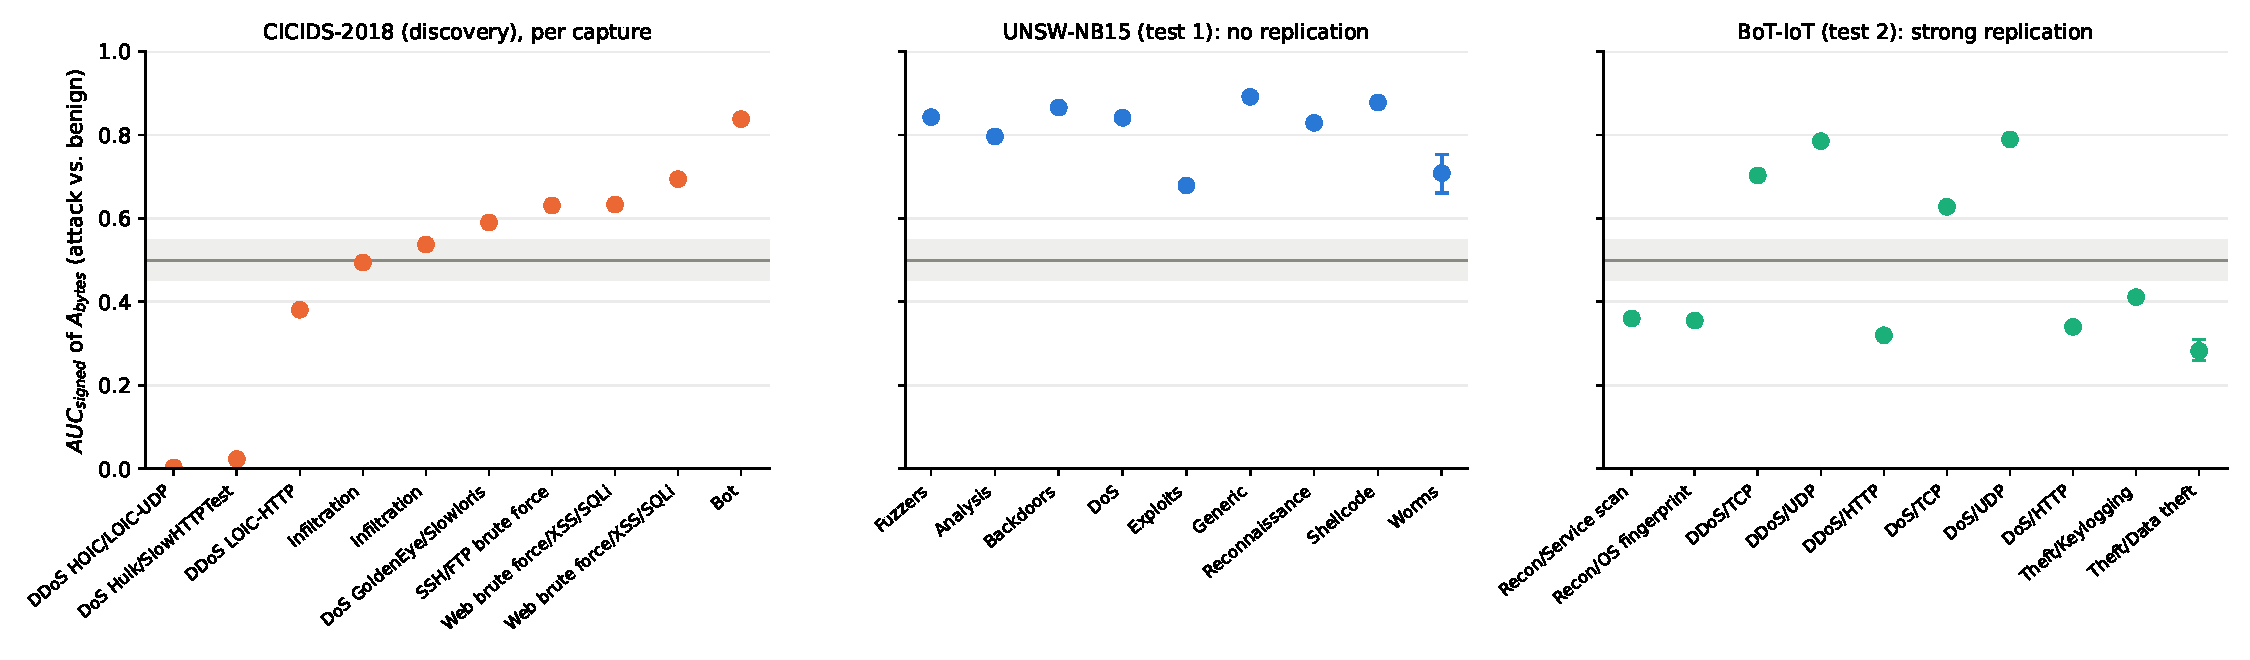
\includegraphics[width=\textwidth]{figures/fig_orientation.pdf}
\caption{$AUC_{signed}$ of $A_{bytes}$ in the discovery analysis and the two preregistered external tests. (a) CICIDS-2018, one point per capture file, each against that capture's own benign flows; exploratory, no CI; each point aggregates every attack label in its capture (per-label values in Table~\ref{tab:cicidslabels}). (b) UNSW-NB15, one point per attack family, in the official family order. (c) BoT-IoT, one point per mechanism group, in the frozen group order. The external tests show the preregistered 95\% stratified flow-level bootstrap CIs ($B=2000$); for BoT-IoT these do not account for host-pair dependence (Table~\ref{tab:a1}). Panel titles give the preregistered verdicts. The gray band is the near-neutral region.\label{fig:orientation}}
\end{figure}

\subsection{UNSW-NB15 (preregistered): no replication}\label{sec:unsw}

All nine families were confidently positive on both features (Table~\ref{tab:unsw}, Figure~\ref{fig:orientation}b), and the script's verdict was \textbf{NO REPLICATION}. The preregistered deduplicated population (2{,}059{,}414 rows) gave the same verdict, with all nine families positive and $A_{bytes}$ between 0.641 and 0.941. The secondary prediction H3-dir failed for DoS, which was positive (0.841), and held for Exploits (0.679). The attacker was the flow source in every attack row of every family, so the attack-oriented variant equals $A_{bytes}$, and $AUC_{sep}=AUC_{signed}$ throughout.

% Source: results/unsw/asymmetry_by_attack.csv (scripts/run_unsw_external_validation.py; code 4d7bc8f/fac0dac, outputs committed in f9b4602).
% W1: three values corrected for double rounding against the CSV (Analysis 0.796472, Exploits A_packets 0.740471, Reconnaissance CI low 0.827480).
\begin{table}[H]
\caption{UNSW-NB15, each family against all Normal flows ($n_{benign} = 2{,}218{,}764$), all rows as released. $A_{bytes}$ and $A_{packets}$ columns give $AUC_{signed}$; 95\% stratified flow-level bootstrap CI for $A_{bytes}$, $B=2000$. \emph{src=att.}: fraction of attack rows whose source is a ground-truth attacker host.\label{tab:unsw}}
\centering
\small
\resizebox{\textwidth}{!}{\begin{tabular}{lrccccc}
\toprule
Family & $n_{attack}$ & $A_{bytes}$ & 95\% CI & $A_{packets}$ & src=att. & Orientation \\
\midrule
Fuzzers        & 24{,}246  & 0.843 & $[0.841, 0.844]$ & 0.881 & 1.00 & positive \\
Analysis       & 2{,}677   & 0.796 & $[0.789, 0.804]$ & 0.902 & 1.00 & positive \\
Backdoors      & 2{,}329   & 0.865 & $[0.860, 0.870]$ & 0.914 & 1.00 & positive \\
DoS            & 16{,}353  & 0.841 & $[0.838, 0.844]$ & 0.898 & 1.00 & positive \\
Exploits       & 44{,}525  & 0.679 & $[0.676, 0.682]$ & 0.740 & 1.00 & positive \\
Generic        & 215{,}481 & 0.891 & $[0.891, 0.892]$ & 0.939 & 1.00 & positive \\
Reconnaissance & 13{,}987  & 0.829 & $[0.827, 0.830]$ & 0.882 & 1.00 & positive \\
Shellcode      & 1{,}511   & 0.878 & $[0.874, 0.882]$ & 0.897 & 1.00 & positive \\
Worms          & 174       & 0.709 & $[0.661, 0.753]$ & 0.724 & 1.00 & positive \\
\bottomrule
\end{tabular}}
\end{table}

\paragraph{Post-hoc observations (not planned; they do not change the verdict)} Most UNSW-NB15 attack flows receive no reply. The fraction of flows with $b_{\leftarrow}=0$ is 0.985 for Generic, 0.834 for Backdoors, 0.777 for DoS and 0.765 for Analysis, against 0.107 for Normal. Analysis, Backdoors and DoS share a sharp step in the empirical distribution at $A_{bytes}\approx 5.30=\log 201$, a fixed-size request with no response bytes (Figure~\ref{fig:ecdf}). Every attack-labeled flow has an attacker host as its source, but 254{,}791 flows labeled Normal (11.5\%) involve an attacker host: 214{,}378 as destination and 40{,}413 as source. Removing them from the benign reference and recomputing every family with the same code, $B$ and seed \emph{raised} every $AUC_{signed}$, by $+0.072$ to $+0.097$, and all nine families remained confidently positive (Table~\ref{tab:labelsens}). The removed flows are themselves source-dominated: flows toward an attacker host are 99.97\% unanswered (median $A_{bytes}=+5.58$), whereas Normal flows that touch no attacker host are unanswered 0.7\% of the time (median $-0.27$). From these observations, and after the verdict, we formulated the reading that orientation is associated with whether the attack's target replies in the capture environment; it became the secondary prediction H3-env of the BoT-IoT freeze (Section~\ref{sec:h3methods}). Under the host-pair cluster bootstrap all nine families remained confidently positive (25--40 attack host pairs per family, 311 benign host pairs), and the Holm correction changed no family's classification.

% Source: results/unsw/posthoc_label_sensitivity.csv (scripts/unsw_posthoc_label_sensitivity.py);
% subset medians: docs/methodology/UNSW_H3_FINDINGS.md POST-HOC item 3. W1: Analysis primary corrected 0.797 -> 0.796 (CSV 0.796472).
\begin{table}[H]
\caption{Post-hoc labeling sensitivity on UNSW-NB15. $AUC_{signed}(A_{bytes})$ against all Normal flows (primary) and against Normal without the 254{,}791 attacker-involved flows ($n_{benign}=1{,}963{,}973$). 95\% bootstrap CI, $B=2000$.\label{tab:labelsens}}
\centering
\small
\resizebox{\textwidth}{!}{\begin{tabular}{lccc}
\toprule
Family & Primary & Normal without attacker hosts & Shift \\
\midrule
Fuzzers        & 0.843 & 0.924 $[0.923, 0.925]$ & $+0.081$ \\
Analysis       & 0.796 & 0.881 $[0.873, 0.889]$ & $+0.085$ \\
Backdoors      & 0.865 & 0.952 $[0.947, 0.957]$ & $+0.087$ \\
DoS            & 0.841 & 0.925 $[0.922, 0.928]$ & $+0.084$ \\
Exploits       & 0.679 & 0.751 $[0.748, 0.754]$ & $+0.072$ \\
Generic        & 0.891 & 0.989 $[0.988, 0.989]$ & $+0.097$ \\
Reconnaissance & 0.829 & 0.922 $[0.920, 0.923]$ & $+0.093$ \\
Shellcode      & 0.878 & 0.953 $[0.950, 0.955]$ & $+0.075$ \\
Worms          & 0.709 & 0.782 $[0.731, 0.831]$ & $+0.073$ \\
\bottomrule
\end{tabular}}
\end{table}

\begin{figure}[H]
\centering
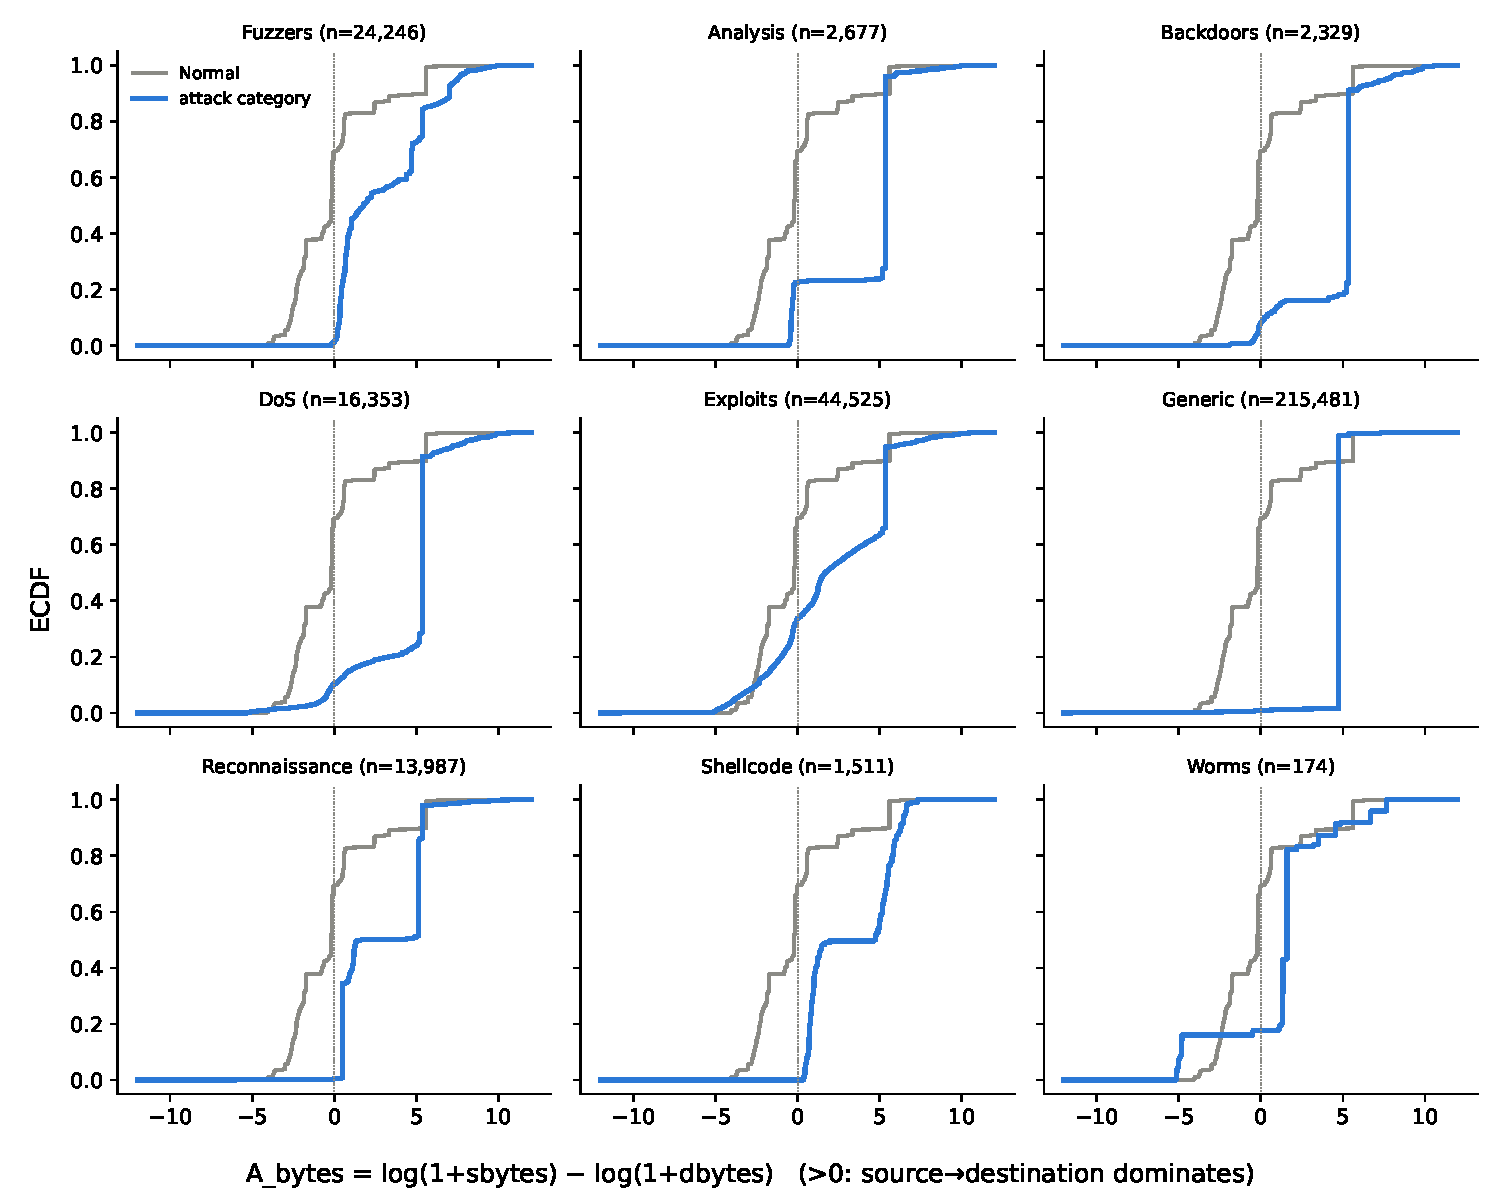
\includegraphics[width=0.9\textwidth]{figures/fig_unsw_ecdf.pdf}
\caption{Empirical distribution of $A_{bytes}$ per UNSW-NB15 family (blue) against Normal (gray). Mass at large positive values corresponds to requests with no response bytes.\label{fig:ecdf}}
\end{figure}

\subsection{BoT-IoT (preregistered): strong replication under the frozen rule}\label{sec:botiot}

The script's verdict was \textbf{STRONG REPLICATION} (Table~\ref{tab:botiot}, Figure~\ref{fig:orientation}c). On $A_{bytes}$ all ten groups were confidently oriented under the preregistered flow-level bootstrap, with opposite signs. The hping3 SYN and UDP floods were positive (0.628--0.789). The scans, the GoldenEye floods and both theft groups were negative (0.283--0.411). The attacker was the flow source in $\ge 96\%$ of rows for every group entering the rule. The criterion also held on $A_{packets}$, where the two GoldenEye groups fell in the near-neutral band (0.460, 0.456). The deduplicated population is identical to the primary one, because BoT-IoT contains no duplicate rows, and gives the same verdict. The Holm correction changed no group's classification.

The secondary predictions separated the two readings. \textbf{H3-env held for all six flood groups}, each confidently. \textbf{H3-dir held for two of seven}: it was right on the two GoldenEye floods, wrong on the four hping3 floods, and wrong on keylogging, which is negative. Keylogging is the one group whose flows mostly have the \emph{victim} as source (75\%), consistent with host-pair labeling and with the reverse connections of the Metasploit scenarios; the role condition keeps it out of the verdict, and its attack-oriented variant is more negative (0.273), not positive. Neither abandonment condition fired.

% Source: results/botiot/asymmetry_by_attack.csv, verdict.json (scripts/run_botiot_h3.py, commit 4554139).
% W1: five values corrected for double rounding against the CSV: DDoS/UDP CI high 0.792482, DoS/TCP CI high 0.635460,
% Keylogging CI high 0.421496, Data theft CI high 0.308500, Data theft C1 0.709467.
\begin{table}[H]
\caption{BoT-IoT, each mechanism group against all Normal flows ($n_{benign}=9{,}543$), all 73{,}370{,}443 rows. Columns $A_{bytes}$, $A_{packets}$ and C1 (size only, $\log(1+b_{\rightarrow}+b_{\leftarrow})$) give $AUC_{signed}$; 95\% preregistered flow-level bootstrap CI for $A_{bytes}$, $B=2000$ (host-pair-aware intervals in Table~\ref{tab:a1}). \emph{src=att.}: fraction of rows whose source is an attacker host. TCP/UDP groups are hping3 floods; HTTP groups are GoldenEye floods. On the flow-level bootstrap every group is confidently oriented: $A_{bytes}<0.5$ negative, $>0.5$ positive. Secondary predictions: \checkmark\ held, $\times$ failed, -- none made.\label{tab:botiot}}
\centering
\footnotesize
\resizebox{\textwidth}{!}{\begin{tabular}{lrccccccc}
\toprule
Group & $n_{attack}$ & $A_{bytes}$ & 95\% CI & $A_{packets}$ & C1 & src=att. & H3-dir & H3-env \\
\midrule
Recon/Service scan   & 1{,}463{,}364  & 0.360 & $[0.351, 0.369]$ & 0.252 & 0.105 & 0.98 & -- & -- \\
Recon/OS fingerprint & 358{,}275      & 0.355 & $[0.346, 0.364]$ & 0.245 & 0.091 & 0.99 & -- & -- \\
DDoS/TCP    & 19{,}547{,}603 & 0.703 & $[0.696, 0.710]$ & 0.714 & 0.583 & 1.00 & $\times$ & \checkmark \\
DDoS/UDP    & 18{,}965{,}106 & 0.785 & $[0.778, 0.792]$ & 0.810 & 0.537 & 1.00 & $\times$ & \checkmark \\
DDoS/HTTP& 19{,}771       & 0.320 & $[0.312, 0.328]$ & 0.460 & 0.713 & 0.97 & \checkmark & \checkmark \\
DoS/TCP     & 12{,}315{,}997 & 0.628 & $[0.621, 0.635]$ & 0.646 & 0.621 & 1.00 & $\times$ & \checkmark \\
DoS/UDP     & 20{,}659{,}491 & 0.789 & $[0.782, 0.797]$ & 0.810 & 0.542 & 1.00 & $\times$ & \checkmark \\
DoS/HTTP & 29{,}706       & 0.340 & $[0.332, 0.349]$ & 0.456 & 0.713 & 0.96 & \checkmark & \checkmark \\
Theft/Keylogging     & 1{,}469        & 0.411 & $[0.401, 0.421]$ & 0.224 & 0.237 & 0.25 & $\times$ & -- \\
Theft/Data theft     & 118            & 0.283 & $[0.259, 0.308]$ & 0.084 & 0.709 & 0.97 & -- & -- \\
\bottomrule
\end{tabular}}
\end{table}

\paragraph{The benign reference, as recorded with the verdict} The BoT-IoT benign reference is 9{,}543 flows produced by a packet generator, 76\% of them UDP~\cite{koroniotis2019botiot}, and a limitation noted in the freeze before any data existed. It is itself strongly source-dominated (median $A_{bytes}=+4.49$, against $-0.22$ for UNSW-NB15's Normal), and 47.3\% of its flows carry reply bytes. In absolute terms the negative groups are mostly balanced: median $A_{bytes}$ is $0.00$ for the scans, $-0.07$ and $+0.01$ for the GoldenEye floods, and $+0.21$ for keylogging. Only data theft is destination-dominated in absolute terms (median $-0.66$). The hping3 floods have medians $0.55$ to $1.69$ above Normal's. The negative orientations are therefore negative relative to this reference, not negative in absolute terms. The C1 column shows that for the scans and the GoldenEye floods, total size separates the classes as well as or better than direction ($AUC_{sep}$ of 0.90--0.91 against 0.64--0.65 for the scans; 0.71 against 0.66--0.68 for GoldenEye). Direction clearly exceeds size only for the hping3 UDP floods ($AUC_{sep}$ 0.79 against 0.54).

\subsection{Post-hoc robustness I: dependence in BoT-IoT (host-pair bootstrap, A1)}\label{sec:a1}

Under the host-pair cluster bootstrap, \textbf{3 of the 8 evaluable BoT-IoT groups retain a confident signed orientation}: DDoS/TCP, DDoS/UDP and DoS/UDP (Table~\ref{tab:a1}). The other five (Recon/Service scan, Recon/OS fingerprint, DDoS/HTTP, DoS/TCP, DoS/HTTP) keep the flow-level sign at the point estimate, but their host-pair intervals include 0.5. They include every negatively oriented group that could be checked. The two theft groups have 6 and 4 host pairs, below the ten-cluster minimum, and are not evaluable. The two-stage bootstrap reproduced every host-pair bound to within 0.013; with hundreds to hundreds of thousands of flows per host pair, resampling flows within pairs adds almost no variance, so it is not an independent check. The three groups confident under host-pair resampling are also confident under the 60\,s time-block bootstrap, the only time-block granularity computable for the floods (21--43 blocks; 3--9 blocks at 300\,s and 600\,s). They are therefore confident under every method computable for them.

% Sources: results/audit/a1_bot_dependence/comparison.csv (flow, hostpair, two_stage, timeblock_60s, cluster_weighted_point),
% results/audit/a1_bot_dependence/benign_concentration.csv (auc_vs_benign_without_dominant_pair), results/dependence/cluster_bootstrap_botiot.csv
\begin{table}[H]
\caption{Post-hoc dependence analysis of BoT-IoT $A_{bytes}$ (A1). 95\% intervals from the flow-level (preregistered), host-pair, two-stage and 60\,s time-block bootstraps ($B=2000$). \emph{Pair-weighted}: point $AUC_{signed}$ with every host pair weighted equally. \emph{w/o top pair}: point $AUC_{signed}$ against the benign reference without its largest host pair (25.2\% of benign flows). \emph{Confident}: confident on the same side under every computable method. n/c: not computable (fewer than ten clusters).\label{tab:a1}}
\centering
\scriptsize
\resizebox{\textwidth}{!}{\begin{tabular}{lcccccccc}
\toprule
Group & Flow & Host pair & Two-stage & Time block 60\,s & Pair-weighted & w/o top pair & Confident \\
\midrule
Recon/Service scan   & $[0.351, 0.369]$ & $[0.214, 0.597]$ & $[0.202, 0.593]$ & $[0.324, 0.405]$ & 0.869 & 0.481 & no \\
Recon/OS fingerprint & $[0.346, 0.364]$ & $[0.200, 0.579]$ & $[0.201, 0.586]$ & $[0.317, 0.394]$ & 0.864 & 0.473 & no \\
DDoS/TCP             & $[0.696, 0.710]$ & $[0.583, 0.854]$ & $[0.587, 0.853]$ & $[0.666, 0.736]$ & 0.924 & 0.721 & yes \\
DDoS/UDP             & $[0.778, 0.792]$ & $[0.634, 0.921]$ & $[0.643, 0.922]$ & $[0.753, 0.814]$ & 0.934 & 0.758 & yes \\
DDoS/HTTP            & $[0.312, 0.328]$ & $[0.166, 0.562]$ & $[0.162, 0.565]$ & $[0.273, 0.362]$ & 0.785 & 0.427 & no \\
DoS/TCP              & $[0.621, 0.635]$ & $[0.487, 0.804]$ & $[0.490, 0.810]$ & $[0.603, 0.652]$ & 0.920 & 0.681 & no \\
DoS/UDP              & $[0.782, 0.797]$ & $[0.641, 0.924]$ & $[0.641, 0.920]$ & $[0.761, 0.816]$ & 0.933 & 0.759 & yes \\
DoS/HTTP             & $[0.332, 0.349]$ & $[0.178, 0.584]$ & $[0.189, 0.588]$ & $[0.303, 0.380]$ & 0.795 & 0.454 & no \\
Theft/Keylogging     & $[0.401, 0.421]$ & n/c (6 pairs) & n/c & $[0.369, 0.453]$ & n/c & 0.549 & not evaluable \\
Theft/Data theft     & $[0.259, 0.308]$ & n/c (4 pairs) & n/c & n/c & n/c & 0.372 & not evaluable \\
\bottomrule
\end{tabular}}
\end{table}

At 60\,s the time-block bootstrap gave a confident interval on the flow-level side for all eight evaluable groups, and at 300\,s and 600\,s for the two Recon groups. The diagnostic run after these results located the source of the disagreement on the benign side. The 9{,}543 benign flows come from 347 host pairs. The largest pair holds 2{,}403 flows (25.2\%), and the five largest hold 45.7\%. That pair's median $A_{bytes}$ ($+5.18$) exceeds 99.7--100\% of the attack flows of the two Recon and the two HTTP groups. Across host-pair replicates its share of the benign reference had a standard deviation of 0.182 (95\% range 0.000--0.557). Across 60\,s time-block replicates the standard deviation was 0.019 (0.214--0.292), because its flows are spread over 201 of the 843 benign 60\,s blocks. Resampling only the benign host pairs, with attack flows fixed, reproduced 89--99\% of the host-pair interval width for every group. Resampling only the attack host pairs left all eight groups confident. The time-block bootstrap holds the dominant benign pair's share nearly constant and so cannot express the uncertainty that host-pair resampling exposes. Its confident intervals for the five groups are not an alternative estimate of the same uncertainty, and the count of evaluable groups with a confident signed orientation is 3 of 8.

Removing the dominant pair from the reference moved the four negatively oriented evaluable groups from 0.320--0.360 to 0.427--0.481 (Table~\ref{tab:a1}). Recon/Service scan (0.481), Recon/OS fingerprint (0.473) and DoS/HTTP (0.454) fall inside the near-neutral band; DDoS/HTTP stays below it (0.427). Theft/Keylogging, which is not evaluable, moved from 0.411 to 0.549, also inside the band. DoS/TCP is a partial exception. The dominant pair lies near the middle of its attack distribution (52.8\% of its attack flows are below the pair's median), benign-only resampling alone gives $[0.520, 0.806]$, and its host-pair interval crosses 0.5 only when attack-side variation is added. Its loss of confidence reflects heterogeneity among benign host pairs in general, and it is marginal. Weighting every host pair equally instead of by its number of flows gave positive point estimates for all eight evaluable groups (0.785--0.934), including the four whose flow-weighted orientation is negative.

For UNSW-NB15, the host-pair bootstrap left all nine families confidently positive (Section~\ref{sec:unsw}). No time-block or two-stage analysis was run for UNSW-NB15.

\subsection{Post-hoc robustness II: reply conditioning (A2)}\label{sec:a2}

\paragraph{BoT-IoT} With both the attack groups and the benign reference restricted to answered flows, all ten BoT-IoT groups have a positive $A_{bytes}$ orientation (0.585--0.953; Table~\ref{tab:a2bot}). The six groups that are negative on all flows (0.283--0.411) become positive (0.585--0.869). For these groups the attack side changes little: the HTTP floods lose 2 flows each, the Recon groups keep 94.2\% and 96.5\% of their flows, and the theft groups keep all of theirs (reply rate 1.000). The benign reference drops from 9{,}543 to its 4{,}514 answered flows. The support for this result differs by group. It rests on the four formerly negative groups with large answered samples (DDoS/HTTP, DoS/HTTP and the two Recon groups, 19{,}769 to 1{,}378{,}580 answered attack flows). The UDP floods' answered slices (406 and 537 flows, 0.002--0.003\% of each group) are too small to represent them, so they were classified on the unanswered slice, which holds more than 99.99\% of their flows: $A_{bytes}$ stays positive but weaker (0.592 and 0.600 against 0.785 and 0.789 on all flows), and the drop comes from restricting the benign side to its 5{,}029 unanswered flows. The theft groups (118 flows from 4 host pairs; 1{,}469 flows from 6) are too small for any dependence check. The two TCP floods, the only groups with large answered and unanswered slices, are positive in both (0.953 and 0.938 answered; 0.605 and 0.643 unanswered).

% Sources: results/audit/a2_reply/auc_by_slice.csv (dataset botiot), results/audit/a2_reply/reply_rates.csv
\begin{table}[H]
\caption{Post-hoc reply conditioning on BoT-IoT (A2). $AUC_{signed}$ of $A_{bytes}$ on all flows, answered flows only and unanswered flows only (same restriction on attack and benign flows; benign $n$ = 9{,}543 / 4{,}514 / 5{,}029), attack $n$ in parentheses; last column $A_{packets}$ on answered flows. Reply rate: fraction of attack flows with reply bytes (benign: 0.473). No CIs (point estimates, see Section~\ref{sec:posthoc-methods}). $^\dagger$~slice too small to represent the group; $^\ddagger$~too few host pairs for any dependence check.\label{tab:a2bot}}
\centering
\scriptsize
\resizebox{\textwidth}{!}{\begin{tabular}{lcccccc}
\toprule
Group & Reply rate & All & Answered & Unanswered & $A_{packets}$ answered \\
\midrule
Recon/Service scan   & 0.942   & 0.360 & 0.745 (1{,}378{,}580) & 0.020 (84{,}784) & 0.499 \\
Recon/OS fingerprint & 0.965   & 0.355 & 0.738 (345{,}635) & 0.067 (12{,}640) & 0.497 \\
DDoS/TCP             & 0.261   & 0.703 & 0.953 (5{,}103{,}403) & 0.605 (14{,}444{,}200) & 0.985 \\
DDoS/UDP             & 0.00002 & 0.785 & 0.780$^\dagger$ (406) & 0.592 (18{,}964{,}700) & 0.607$^\dagger$ \\
DDoS/HTTP            & 0.9999  & 0.320 & 0.676 (19{,}769) & --$^\dagger$ (2) & 0.966 \\
DoS/TCP              & 0.500   & 0.628 & 0.938 (6{,}152{,}453) & 0.643 (6{,}163{,}544) & 0.992 \\
DoS/UDP              & 0.00003 & 0.789 & 0.775$^\dagger$ (537) & 0.600 (20{,}658{,}954) & 0.593$^\dagger$ \\
DoS/HTTP             & 0.9999  & 0.340 & 0.719 (29{,}704) & --$^\dagger$ (2) & 0.957 \\
Theft/Keylogging     & 1.000   & 0.411 & 0.869$^\ddagger$ (1{,}469) & -- (0) & 0.473$^\ddagger$ \\
Theft/Data theft     & 1.000   & 0.283 & 0.585$^\ddagger$ (118) & -- (0) & 0.171$^\ddagger$ \\
\bottomrule
\end{tabular}}
\end{table}

$A_{packets}$ does not follow $A_{bytes}$ uniformly on the answered slice. Data theft stays negative (0.171), and the two Recon groups (0.497, 0.499) and keylogging (0.473) are near-neutral. On the unanswered slice, the minority of Recon flows without a reply (5.8\% of Service scan and 3.5\% of OS fingerprint) are strongly negative (0.020, 0.067), while the TCP and UDP floods are 0.592--0.643: among unanswered flows, the magnitude of $A_{bytes}$ separates the Recon groups from the floods.

A2's four sign flips among evaluable groups are four of the five groups that lose confidence under host-pair resampling. The fifth, DoS/TCP, persists and strengthens under A2 (0.628 to 0.938). In the pre-committed A1$\times$A2 matrix, DDoS/TCP falls in the cell ``survives, survives''; DDoS/UDP and DoS/UDP in the same cell but with a weakened unanswered-slice value; DoS/TCP in ``weakens, survives'' (the phenomenon exists and the original interval overstated its precision); and the four formerly negative groups in ``weakens, collapses or flips'', which the matrix labels a benchmark-interaction or reply-structure artifact. A1 and A2 act on the same flows and on the same 9{,}543-flow benign reference, whose reply mix and host-pair concentration both change the comparison. Their agreement is expected from that shared structure and is not independent corroboration.

\paragraph{UNSW-NB15} Reply conditioning changes fewer UNSW-NB15 readings, but not none (Table~\ref{tab:a2unsw}). Eight of the nine families persist: they keep a positive orientation outside the band on their answered flows, several with a higher value (Fuzzers 0.883, Reconnaissance 0.848, Shellcode 0.909). Generic persists only weakly: it drops from 0.891 to 0.561 on 3{,}247 answered flows, 0.061 above 0.5 and so just outside the band, and those flows are only 1.5\% of the family, an unrepresentative slice. \textbf{Analysis is the one collapse}: it falls from 0.796 to 0.506 on 630 answered flows, which comprise 23.5\% of the family and constitute a substantially less sparse conditioned slice than Generic's 1.5\%. $A_{packets}$ persists on the answered slice for all nine families, including Analysis (0.842).

On the unanswered slice the UNSW-NB15 values are reported but not classified (Table~\ref{tab:a2unsw}, last column). Six families are strongly negative there (0.045--0.177) and Fuzzers is 0.432; Shellcode (0.475) is in the band, and Worms has 21 unanswered flows. Read against the band alone, seven families would be flips. This slice is not reply-conditioning evidence of the kind the answered slice gives, because of what its benign reference contains. Its 238{,}359 Normal flows are the unanswered Normal flows, and by the subset shares recorded with the labeling-sensitivity analysis (Section~\ref{sec:unsw}; no reply bytes in 99.97\% of the 214{,}378 Normal flows toward an attacker host, 25.4\% of the 40{,}413 from one, and 0.7\% of the 1{,}963{,}973 that touch none) about 94\% of them involve an attacker host. The unanswered comparison therefore sets attack flows mainly against attacker-involved flows labeled Normal, the population whose removal raised every family's all-flows value (Table~\ref{tab:labelsens}). The A2 report does not classify this slice, and we do not use it as evidence in either direction.

% Sources: results/audit/a2_reply/auc_by_slice.csv (dataset unsw), results/audit/a2_reply/reply_rates.csv
% ~94% attacker-involved: arithmetic on the subset table in docs/methodology/UNSW_H3_FINDINGS.md POST-HOC item 3
% (214,378 x 0.9997 + 40,413 x 0.254 = 224,579 of 238,359 = 0.942; the 0.007 share rounded +/-0.0005 gives 93.8-94.6%).
\begin{table}[H]
\caption{Post-hoc reply conditioning on UNSW-NB15 (A2). $AUC_{signed}$ of $A_{bytes}$ on all flows, on answered flows only and on unanswered flows only (attack $n$ in parentheses; benign $n$ = 2{,}218{,}764 / 1{,}980{,}405 / 238{,}359, benign reply rate 0.893), and $A_{packets}$ on answered flows. No CIs. Class: A2 classification of the answered slice. $^\ddagger$~answered slice is 1.5\% of the family (unrepresentative). The unanswered slice is not classified: its benign reference is about 94\% attacker-involved flows labeled Normal (see text).\label{tab:a2unsw}}
\centering
\footnotesize
\resizebox{\textwidth}{!}{\begin{tabular}{lcccccc}
\toprule
Family & Reply rate & All & Answered & Class & $A_{packets}$ answered & Unanswered \\
\midrule
Fuzzers        & 0.639 & 0.843 & 0.883 (15{,}503) & persists & 0.935 & 0.432 (8{,}743) \\
Analysis       & 0.235 & 0.796 & 0.506 (630) & \textbf{collapses} & 0.842 & 0.094 (2{,}047) \\
Backdoors      & 0.166 & 0.865 & 0.729 (386) & persists & 0.819 & 0.145 (1{,}943) \\
DoS            & 0.223 & 0.841 & 0.678 (3{,}646) & persists & 0.798 & 0.149 (12{,}707) \\
Exploits       & 0.631 & 0.679 & 0.608 (28{,}102) & persists & 0.686 & 0.177 (16{,}423) \\
Generic        & 0.015 & 0.891 & 0.561 (3{,}247) & persists (weak)$^\ddagger$ & 0.614 & 0.045 (212{,}234) \\
Reconnaissance & 0.502 & 0.829 & 0.848 (7{,}017) & persists & 0.916 & 0.083 (6{,}970) \\
Shellcode      & 0.496 & 0.878 & 0.909 (750) & persists & 0.949 & 0.475 (761) \\
Worms          & 0.879 & 0.709 & 0.754 (153) & persists & 0.776 & 0.671 (21) \\
\bottomrule
\end{tabular}}
\end{table}

\subsection{Post-hoc robustness III: CICIDS-2018 labels, benign reference and degenerate measurements (A2, A3)}\label{sec:cicids-audit}

\paragraph{Labels} The ten capture files contain 14 distinct attack labels (Table~\ref{tab:cicidslabels}). No label merges two attack tools, and no attack label collapses into the benign class. The attack-count-weighted mean of the per-label values in each capture reproduces all ten per-capture values of Section~\ref{sec:discovery} to three decimals, which is exact because all labels in a capture share one benign reference. For the HOIC/LOIC-UDP capture, $(668{,}461\times 0.0005 + 1{,}730\times 1.000)/670{,}191 = 0.003$. That capture's value is thus almost entirely HOIC (99.7\% of its attack flows), and its two labels have opposite orientations.

% Sources: results/audit/a3_cicids_labels.csv (per-capture), results/audit/a2_reply/auc_by_slice.csv (dataset cicids; slices all, answered),
% results/audit/a2_reply/reply_rates.csv; unanswered slice (0.382706, 4,076,376 benign) cited in text only. Answered-only HOIC 0.242529 printed as 0.243 (the A2 report text truncates to 0.242).
% The six-label "unanswered A_bytes exactly 0" set (HOIC, Hulk, SlowHTTPTest, FTP-BruteForce, SSH-Bruteforce, SQL Injection) is
% docs/reviewer_audit/A2_REPLY_CONDITIONAL_REPORT.md, "Diagnostic follow-up" (~lines 106-125): an ad hoc check, not a committed CSV
% column, cross-checked here against auc_by_slice.csv's identical 0.382705618912485 for all six and, for HOIC/Hulk specifically,
% against A4's independently-derived row-level zero-payload counts (504,711 / 409,325), which match exactly.
\begin{table}[H]
\caption{Post-hoc CICIDS-2018 per-label audit (A2, A3). $AUC_{signed}$ of $A_{bytes}$ against each capture's own benign flows (per capture; two values for labels present in two captures) and against all 13{,}467{,}970 benign flows pooled (all flows; answered flows only, attack $n$ in parentheses). Reply rates of attack flows by bytes and by packets (benign: 0.697 and 0.800). $^\ast$~exactly constant $A_{bytes}=0$ on every attack flow. $^\dagger$~fewer than 1{,}000 attack flows. No CIs.\label{tab:cicidslabels}}
\centering
\scriptsize
\resizebox{\textwidth}{!}{\begin{tabular}{lrcccccc}
\toprule
Label & $n$ & Reply (bytes) & Reply (packets) & Per capture & Pooled, all & Pooled, answered \\
\midrule
DDOS attack-HOIC             & 668{,}461 & 0.245 & 0.245 & 0.0005 & 0.577 & 0.243 (163{,}750) \\
DDOS attack-LOIC-UDP         & 1{,}730   & 0.000 & 0.000 & 1.000  & 1.000 & -- (0) \\
DDoS attacks-LOIC-HTTP       & 576{,}191 & 0.502 & 0.502 & 0.381  & 0.357 & 0.010 (289{,}289) \\
DoS attacks-Hulk             & 434{,}873 & 0.059 & 0.059 & 0.023  & 0.681 & 0.329 (25{,}548) \\
DoS attacks-SlowHTTPTest$^\ast$ & 19{,}462 & 0.000 & 1.000 & 0.025 & 0.709 & -- (0) \\
DoS attacks-GoldenEye        & 41{,}455  & 0.647 & 0.670 & 0.510  & 0.467 & 0.450 (26{,}807) \\
DoS attacks-Slowloris        & 10{,}285  & 0.014 & 0.773 & 0.912  & 0.904 & 0.284 (142) \\
Bot                          & 282{,}310 & 0.506 & 0.507 & 0.838  & 0.779 & 0.893 (142{,}865) \\
Infilteration                & 161{,}897 & 0.562 & 0.845 & 0.537 / 0.494 & 0.511 & 0.436 (90{,}956) \\
FTP-BruteForce$^\ast$        & 39{,}352  & 0.000 & 1.000 & 0.761  & 0.709 & -- (0) \\
SSH-Bruteforce               & 117{,}322 & 0.800 & 1.000 & 0.588  & 0.528 & 0.692 (93{,}818) \\
Brute Force -Web$^\dagger$   & 611       & 0.439 & 0.445 & 0.817 / 0.708 & 0.760 & 0.828 (268) \\
Brute Force -XSS$^\dagger$   & 230       & 0.491 & 0.496 & 0.454 / 0.447 & 0.441 & 0.221 (113) \\
SQL Injection$^\dagger$      & 87        & 0.552 & 0.667 & 0.536 / 0.513 & 0.508 & 0.418 (48) \\
\bottomrule
\end{tabular}}
\end{table}

\paragraph{Benign reference} Scored against the benign flows of their own capture, HOIC, Hulk and SlowHTTPTest are negative (0.0005, 0.023, 0.025). Scored against the pooled benign flows, the same attack flows are positive (0.577, 0.681, 0.709). Their two captures are the only ones whose own benign median $A_{bytes}$ is positive (1.105 for HOIC's capture, 0.975 for Hulk's and SlowHTTPTest's); in the other captures it lies between $-0.34$ and $-0.30$. Elsewhere no confident orientation changes side between the two conventions; GoldenEye (0.510 per capture, 0.467 pooled) and the Wednesday 28-02 infiltration capture (0.494, against 0.511 pooled over both infiltration captures) move across 0.5 within the near-neutral band.

\paragraph{Degenerate measurements} Three labels do not support a magnitude reading of $A_{bytes}$. All LOIC-UDP flows are unanswered by bytes and by packets, so its value of 1.000 cannot be separated from the absence of replies. Every one of the 19{,}462 SlowHTTPTest flows and the 39{,}352 FTP-BruteForce flows has one forward and one backward packet and no payload in either direction, so their $A_{bytes}$ is exactly 0 on every flow, with zero variance. Their $AUC_{signed}$ values (0.709 pooled; 0.025 and 0.761 per capture) are determined entirely by where the benign reference lies relative to 0; the pooled benign median is $-0.320$ and 17.4\% of pooled benign flows are above 0. These values carry no information about variation in the attack traffic. For the same two labels the reply rate is 0 by bytes and 1.000 by packets: under CICFlowMeter's payload-only accounting, a backward direction that carries only header packets counts as unanswered. Byte-based and packet-based reply rates differ for 10 of the 14 labels and for the benign flows, whereas they are identical for every UNSW-NB15 and BoT-IoT group.

\paragraph{Reply conditioning} Against the pooled reference, HOIC and Hulk are positive on all flows and negative on their answered flows (0.243 and 0.329, on 163{,}750 and 25{,}548 attack flows), which agrees with their per-capture sign; $A_{packets}$ moves the same way (0.057, 0.157). LOIC-HTTP is negative on all flows and more so on answered flows (0.357, 0.010). SSH-Bruteforce is near-neutral on all flows and positive on answered flows (0.528, 0.692). Slowloris's answered slice has 142 flows. LOIC-UDP, SlowHTTPTest and FTP-BruteForce have no answered flows by bytes. The unanswered slice is not interpreted for CICIDS-2018: for HOIC, Hulk, SlowHTTPTest, FTP-BruteForce, SSH-Bruteforce and SQL Injection, every unanswered attack flow carries no bytes in either direction, so $A_{bytes}$ is exactly 0 and all six labels receive the same value (0.383) against the shared 4{,}076{,}376 unanswered benign flows.

\subsection{Post-hoc robustness IV: the same traffic under a different flow representation (A4)}\label{sec:a4}

A4 compares the canonical CICFlowMeter representation of CICIDS-2018 with its NetFlow-v2 re-export, label by label, each against its own global benign reference (Table~\ref{tab:a4}). The integrity gates passed, and the new pipeline reproduced all 171 committed canonical values before any NetFlow-v2 number was computed. A4 concerns CICIDS-2018 only.

% Sources: results/audit/a4_representation/fine_label_auc.csv (feature A_bytes), comparison.csv, reply_rates.csv,
% run_summary.json (case_primary_A_bytes = C). Frozen protocol: docs/reviewer_audit/A4_REPRESENTATION_SENSITIVITY.md at 946337f.
\begin{table}[H]
\caption{Post-hoc same-traffic representation analysis (A4), $A_{bytes}$, the 11 well-supported labels. Each representation against its own global benign reference (canonical CICFlowMeter: 13{,}467{,}970 flows, byte reply rate 0.697; NetFlow-v2: 16{,}635{,}567 flows, 0.931). Reply: fraction of attack flows with reply bytes. No CIs; statuses from point estimates and the near-neutral band. $^\ast$~canonical $A_{bytes}$ exactly 0 on every flow (Section~\ref{sec:cicids-audit}). Under-supported, reported only: Brute Force -Web (611/2{,}143 flows; 0.760 to 0.309), -XSS (230/927; 0.441 to 0.247), SQL Injection (87/432; 0.508 to 0.252).\label{tab:a4}}
\centering
\scriptsize
\resizebox{\textwidth}{!}{\begin{tabular}{lrrcccccl}
\toprule
 & \multicolumn{2}{c}{$n_{attack}$} & \multicolumn{2}{c}{$AUC_{signed}$} & \multicolumn{2}{c}{$AUC_{sep}$} & Reply & \\
Label & canonical & NF-v2 & can. & NF-v2 & can. & NF-v2 & can.\,/\,NF-v2 & Status \\
\midrule
DDOS attack-HOIC         & 668{,}461 & 1{,}080{,}858 & 0.577 & 0.223 & 0.577 & 0.777 & 0.245 / 1.000 & \textbf{REVERSED} \\
DDOS attack-LOIC-UDP     & 1{,}730   & 2{,}112   & 1.000 & 1.000 & 1.000 & 1.000 & 0.000 / 0.000 & PRESERVED \\
DDoS attacks-LOIC-HTTP   & 576{,}191 & 307{,}300 & 0.357 & 0.129 & 0.643 & 0.871 & 0.502 / 0.912 & PRESERVED \\
DoS attacks-Hulk         & 434{,}873 & 432{,}648 & 0.681 & 0.349 & 0.681 & 0.651 & 0.059 / 0.9996 & \textbf{REVERSED} \\
DoS attacks-SlowHTTPTest$^\ast$ & 19{,}462 & 14{,}116 & 0.709 & 0.875 & 0.709 & 0.875 & 0.000 / 1.000 & PRESERVED \\
DoS attacks-GoldenEye    & 41{,}455  & 27{,}723  & 0.467 & 0.509 & 0.533 & 0.509 & 0.647 / 1.000 & BOTH NEUTRAL \\
DoS attacks-Slowloris    & 10{,}285  & 9{,}512   & 0.904 & 0.939 & 0.904 & 0.939 & 0.014 / 0.760 & PRESERVED \\
Bot                      & 282{,}310 & 143{,}097 & 0.779 & 0.873 & 0.779 & 0.873 & 0.506 / 1.000 & PRESERVED \\
Infilteration            & 161{,}897 & 116{,}361 & 0.511 & 0.483 & 0.511 & 0.517 & 0.562 / 0.983 & BOTH NEUTRAL \\
FTP-BruteForce$^\ast$    & 39{,}352  & 25{,}933  & 0.709 & 0.875 & 0.709 & 0.875 & 0.000 / 1.000 & PRESERVED \\
SSH-Bruteforce           & 117{,}322 & 94{,}979  & 0.528 & 0.707 & 0.528 & 0.707 & 0.800 / 1.000 & EMERGED \\
\bottomrule
\end{tabular}}
\end{table}

\paragraph{Primary result} Of the 11 well-supported labels, 8 have a confident canonical orientation. \textbf{Two of these 8 reverse under NetFlow-v2}: HOIC ($AUC_{signed}$ 0.577 to 0.223) and Hulk (0.681 to 0.349). Six labels are preserved (LOIC-UDP, LOIC-HTTP, SlowHTTPTest, Slowloris, Bot, FTP-BruteForce), SSH-Bruteforce emerges (0.528 to 0.707), GoldenEye and Infilteration are near-neutral in both representations, and none is neutralized. Two of 8 is below the frozen Case~D threshold of at least 5 of 8, so the pre-committed aggregate reading is \textbf{Case~C}: the signed orientation of at least one mechanism differs between the two representation-plus-reference pairs. On $A_{packets}$, for which no case is assigned, HOIC also reverses (0.671 to 0.355) and Hulk is preserved (0.844 to 0.616).

\paragraph{What changes together (C2)} The comparison changes more than the flow exporter. The two global benign references are different populations (13{,}467{,}970 and 16{,}635{,}567 flows, with byte-based reply rates 0.697 and 0.931), and they cannot be capture-matched because the NetFlow-v2 file has no timestamp or capture field. Flow segmentation (the flow count differs for every label), byte accounting (payload only against whole packets), the source-endpoint rule (unverified) and possibly label assignment change with it. Matching fine labels controls only the composition of the attack side. The reversals are therefore properties of the representation-plus-reference pair. A4 does not attribute them to the exporter or to any single factor.

\paragraph{Separability} The reversals did not eliminate discriminative separation. HOIC's $AUC_{sep}$ increased from 0.577 to 0.777, whereas Hulk's decreased modestly from 0.681 to 0.651. (That both values exceed 0.55 follows from the REVERSED status itself, Section~\ref{sec:auc}, and is not evidence; the magnitudes are the information.) $AUC_{sep}$ increased by at least 0.05 under NetFlow-v2 for HOIC, LOIC-HTTP, SlowHTTPTest, Bot, FTP-BruteForce and SSH-Bruteforce.

\paragraph{Constant-valued labels} Two of the six preserved labels, SlowHTTPTest and FTP-BruteForce, are the constant-valued labels of Section~\ref{sec:cicids-audit}. Their canonical $A_{bytes}$ is constant and contains no attack-side variation, so their canonical orientation (0.709) is a statement about the canonical benign reference only, and their ``preservation'' cannot be read as evidence of stable attack-side orientation. They remain in the frozen denominator and are not reclassified. As a post-hoc sensitivity, excluding them leaves 6 canonical-confident labels, of which 2 reverse; Case~D would require at least 4 of 6, so the reading remains Case~C. This check does not redefine the frozen case.

\paragraph{Row-level composition of HOIC and Hulk (post-hoc, descriptive)} In neither representation are HOIC or Hulk flows forward-dominant in absolute terms: the fraction with $A_{bytes}>0$ is at most 0.35\% on either side. A check of the raw rows, outside the frozen outputs, found that 504{,}711 of the 668{,}461 canonical HOIC flows (75.5\%) are short unidirectional records with exactly two forward packets, no backward packets and no payload in either direction, so their $A_{bytes}$ is exactly 0. The same holds for 409{,}325 of the 434{,}873 canonical Hulk flows (94.1\%, with two or three forward packets). These records lie above the canonical benign median ($-0.320$), and the canonical positive orientation of both labels is dominated by them. The canonical flows that do carry a reply lie below the benign median: median $A_{bytes}$ $-1.11$ for HOIC, with all of these flows below the benign median, and $-0.98$ for Hulk, with 96.3\% below it. Under NetFlow-v2 such records are essentially absent. Every HOIC flow and 99.96\% of Hulk flows carry a reply, with median $A_{bytes}$ of $-0.79$ and $-0.62$ against a benign median of $-0.29$. The benign reference's median and share of positive values moved little between the representations ($-0.320$ to $-0.288$; 0.174 to 0.162; this does not exclude that the two benign references differ in other respects, C2, see the next paragraph), whereas the composition of the attack flows changed.

\paragraph{Byte accounting does not account for the reversal} The zero-payload records have no backward packets, and therefore no backward bytes under either accounting convention. Their $A_{bytes}$ is thus non-negative under either convention: exactly 0 under payload-only accounting, and strictly positive if headers are counted, as NetFlow-v2 does. Counting headers on those same records would move them further above the benign reference and strengthen the canonical positive orientation rather than reverse it. The row-level evidence instead points to differences in how the two pipelines construct and segment flows for these attacks. The evidence is descriptive: because the benign references differ (C2) and label assignment may differ, it does not isolate flow construction as the cause.

\paragraph{Coarse categories and attack-only contrasts} When labels are pooled into coarse categories, the orientation depends on how the sub-labels are weighted. With identical weights on both sides, DDoS and DoS $A_{bytes}$ change status with the weighting convention: DoS reads REVERSED under either representation's row shares but PRESERVED under equal weights per label, and DDoS reads EMERGED under row shares but NEUTRALIZED under equal weights. Raw pooling would report DDoS as EMERGED (0.475 to 0.203), a status that none of its sub-labels shows. The benign-free contrast between LOIC-UDP and HOIC, which share a canonical capture, is 1.000 in both representations, and none of the four same-capture label contrasts reverses; the canonical SlowHTTPTest--Hulk contrast is 94.1\% ties at $A_{bytes}=0$.

\subsection{Orientation and separation across the analyses}\label{sec:orientsep}

Table~\ref{tab:orientsep} collects the cases above in which a change of benign reference, host-pair weighting, reply slice or representation moved $AUC_{signed}$ to the other side of 0.5 or into the near-neutral band, with $AUC_{sep}$ before and after. It omits cases already excluded as evidence above: the constant-valued SlowHTTPTest and FTP-BruteForce, labels with fewer than 1{,}000 attack flows or a conditioned slice of fewer than 1{,}000 flows (for example Slowloris answered, 142 flows), the unclassified unanswered slices of UNSW-NB15 and CICIDS-2018 (Sections~\ref{sec:a2} and~\ref{sec:cicids-audit}), moves across 0.5 that stay inside the band (GoldenEye, Infilteration), and moves out of the band (SSH-Bruteforce, pooled all to answered flows and canonical to NetFlow-v2; Infilteration, pooled all to answered flows, 0.511 to 0.436). UNSW-NB15 Generic (0.891 to 0.561 on a 1.5\% answered slice) is not listed: it persists, weakly, dropping sharply but staying outside the band on the same side. The upper block of the table lists sixteen sign changes between two values outside the band, six for CICIDS-2018 and ten for BoT-IoT. $AUC_{sep}$ after the change lies between 0.577 and 0.777 for the six CICIDS-2018 changes (reference, reply slice and representation) and between 0.585 and 0.869 for the ten BoT-IoT changes (reply slice and host-pair weighting); the two datasets are not pooled here because the changes and the benign references differ. Because each sign change is between two values outside the band, $AUC_{sep}\ge 0.55$ on both sides holds by construction; the magnitudes are the information. The magnitude rose in some cases (HOIC, canonical to NetFlow-v2: 0.577 to 0.777; Recon/Service scan, flow- to pair-weighted: 0.640 to 0.869) and fell sharply in others (HOIC, per-capture to pooled reference: 0.9995 to 0.577). Moves into the band are different: removing the dominant benign host pair lowered the separation of the three evaluable groups that entered the band to 0.519--0.546 (DDoS/HTTP, which stayed outside the band at 0.427, is not listed), the change from per-capture to pooled reference lowered that of SSH-Bruteforce from 0.588 to 0.528, and reply conditioning removed both the orientation and the separation of UNSW-NB15 Analysis (0.796 to 0.506).

% Sources: every value is copied from a table above (tab:cicidslabels, tab:a4, tab:a2bot, tab:a1, tab:a2unsw) or from the
% committed files named there; AUC_sep = max(x, 1-x) of those values. Nothing is recomputed from data.
\begin{table}[H]
\caption{Orientation ($AUC_{signed}$) and separation ($AUC_{sep}$) of $A_{bytes}$ before and after each change of reference, host-pair weighting, reply slice or representation that moved $AUC_{signed}$ across 0.5 or into the near-neutral band. Upper block: sign changes between two values outside the band; lower block: moves into the band (Theft/Keylogging also crosses 0.5). All changes are post-hoc; the ``before'' values of the CICIDS per-capture rows are exploratory and those of the BoT-IoT rows are the preregistered flow-level estimates. Pair-weighted: every host pair weighted equally (A1, Table~\ref{tab:a1}). Theft rows are kept, flagged, because they belong to the preregistered groups, although they have too few host pairs and the Data theft slice has 118 flows. $^\dagger$~too few host pairs for any dependence check.\label{tab:orientsep}}
\centering
\scriptsize
\resizebox{\textwidth}{!}{\begin{tabular}{llcccc}
\toprule
 & & \multicolumn{2}{c}{$AUC_{signed}$} & \multicolumn{2}{c}{$AUC_{sep}$} \\
Group & Change & before & after & before & after \\
\midrule
CICIDS HOIC   & per-capture $\to$ pooled benign & 0.0005 & 0.577 & 0.9995 & 0.577 \\
CICIDS Hulk   & per-capture $\to$ pooled benign & 0.023  & 0.681 & 0.977 & 0.681 \\
CICIDS HOIC   & pooled: all $\to$ answered flows & 0.577 & 0.243 & 0.577 & 0.757 \\
CICIDS Hulk   & pooled: all $\to$ answered flows & 0.681 & 0.329 & 0.681 & 0.671 \\
CICIDS HOIC   & canonical $\to$ NetFlow-v2 (A4) & 0.577 & 0.223 & 0.577 & 0.777 \\
CICIDS Hulk   & canonical $\to$ NetFlow-v2 (A4) & 0.681 & 0.349 & 0.681 & 0.651 \\
BoT-IoT DDoS/HTTP & all $\to$ answered flows & 0.320 & 0.676 & 0.680 & 0.676 \\
BoT-IoT DoS/HTTP  & all $\to$ answered flows & 0.340 & 0.719 & 0.660 & 0.719 \\
BoT-IoT Recon/Service scan & all $\to$ answered flows & 0.360 & 0.745 & 0.640 & 0.745 \\
BoT-IoT Recon/OS fingerprint & all $\to$ answered flows & 0.355 & 0.738 & 0.645 & 0.738 \\
BoT-IoT Theft/Keylogging$^\dagger$ & all $\to$ answered flows & 0.411 & 0.869 & 0.589 & 0.869 \\
BoT-IoT Theft/Data theft$^\dagger$ & all $\to$ answered flows & 0.283 & 0.585 & 0.717 & 0.585 \\
BoT-IoT Recon/Service scan & flow- $\to$ pair-weighted & 0.360 & 0.869 & 0.640 & 0.869 \\
BoT-IoT Recon/OS fingerprint & flow- $\to$ pair-weighted & 0.355 & 0.864 & 0.645 & 0.864 \\
BoT-IoT DDoS/HTTP & flow- $\to$ pair-weighted & 0.320 & 0.785 & 0.680 & 0.785 \\
BoT-IoT DoS/HTTP  & flow- $\to$ pair-weighted & 0.340 & 0.795 & 0.660 & 0.795 \\
\midrule
BoT-IoT DoS/HTTP & without dominant benign pair & 0.340 & 0.454 & 0.660 & 0.546 \\
BoT-IoT Recon/Service scan & without dominant benign pair & 0.360 & 0.481 & 0.640 & 0.519 \\
BoT-IoT Recon/OS fingerprint & without dominant benign pair & 0.355 & 0.473 & 0.645 & 0.527 \\
BoT-IoT Theft/Keylogging$^\dagger$ & without dominant benign pair & 0.411 & 0.549 & 0.589 & 0.549 \\
CICIDS SSH-Bruteforce & per-capture $\to$ pooled benign & 0.588 & 0.528 & 0.588 & 0.528 \\
UNSW Analysis & all $\to$ answered flows & 0.796 & 0.506 & 0.796 & 0.506 \\
\bottomrule
\end{tabular}}
\end{table}

% =====================================================================
\section{Extended discussion and limitations}\label{sec:discussion}
% =====================================================================
% Rewrite, phase W2 (2026-09-27). Written against manuscript/rewrite/WRITING_EVIDENCE_CONTRACT.md,
% docs/methodology/CLAIMS_LEDGER.md and docs/reviewer_audit/AUDIT_SYNTHESIS.md, and against the frozen
% W1 Methods/Results. Every number below is copied from Section sec:results.

\subsection{What the results establish}\label{sec:disc-established}

The analyses were run in a fixed order, and the evidence they provide differs in kind (Table~\ref{tab:chronology}). Read in that order, they establish the following.

\begin{enumerate}
\item \textbf{H2 was rejected.} Under Bernoulli flow sampling and window truncation, graph topology did not degrade less than per-flow directional asymmetry, on the synthetic generator or on the one real capture with IP addresses (Section~\ref{sec:h2}). The closest real-data case, 1:100 sampling, favored topology by less than the preregistered margin. The result is scoped to those two operators and those two instruments. It does not show that topology is uninformative in general.
\item \textbf{The CICIDS-2018 observation did not replicate on UNSW-NB15.} In the preregistered test, all nine UNSW-NB15 families were confidently positive, and the secondary prediction that its DoS family would be inverted failed (Section~\ref{sec:unsw}). This is the first external result on H3, and it is negative.
\item \textbf{BoT-IoT met the frozen criterion, and its interpretation is substantially weaker than its verdict suggests.} Under the preregistered flow-level rule, BoT-IoT gave STRONG REPLICATION, and the reading formulated after UNSW-NB15 (H3-env) predicted all six flood groups in advance (Section~\ref{sec:botiot}). That verdict stands as the output of the frozen rule. The post-hoc analyses change what it can be taken to mean. Only 3 of the 8 evaluable groups keep a confident signed orientation under host-pair-aware resampling, and every checkable negatively oriented group loses its confidence (Section~\ref{sec:a1}). With reply presence held fixed, or with host pairs weighted equally, no evaluable group remains negative on $A_{bytes}$ (Sections~\ref{sec:a1} and~\ref{sec:a2}). All ten answered-only point estimates are positive, although the UDP-flood answered slices (406 and 537 flows) and the Theft groups are too sparse for strong inference; among the adequately supported formerly negative groups, the negative orientation disappears. The ``some groups positive, some confidently negative'' pattern that constitutes the replication therefore depends on how the small benign reference is composed and weighted.
\item \textbf{The CICIDS-2018 observation is a composite of resolvable labels measured against a particular reference.} Each per-capture value is the flow-weighted mean of distinct labels (Section~\ref{sec:cicids-audit}). The most extreme capture value, 0.003, is the count-weighted aggregate of HOIC (0.0005) and LOIC-UDP (1.000), dominated numerically by HOIC; it should not be read as the orientation of a single attack mechanism. Three labels change side when scored against pooled rather than per-capture benign flows, and two labels (SlowHTTPTest, FTP-BruteForce) have constant $A_{bytes}=0$ and carry no attack-side variation.
\item \textbf{Within the same underlying CICIDS-2018 capture environment, a different representation-plus-reference pair reversed two fine-label orientations.} Two of the 8 well-supported labels with confident canonical orientation, HOIC and Hulk, reverse under the NetFlow-v2 re-export with its own benign reference (Case~C; Section~\ref{sec:a4}). Six labels keep their orientation, two of them only in the sense that a constant attack value was read against a different benign distribution. The two benign references cannot be matched (C2), so the reversal is a property of the pair, not of the exporter alone.
\end{enumerate}

None of these results supports the hypothesis that attack mechanism determines the sign of directional asymmetry. The CICIDS mechanism reading (H3-dir) held for 2 of 7 BoT-IoT predictions, the UNSW-NB15 test found no inversion at all, and the CICIDS labels on which the reading was based change side with the benign reference and, for HOIC and Hulk, with the representation-plus-reference pair.

\subsection{Signed orientation as a relational measurement}\label{sec:disc-relational}

$AUC_{signed}$ compares two distributions: the probability that an attack flow's $A$ exceeds a benign flow's $A$. Its sign is therefore a property of an attack population, a benign reference population and the measurement pipeline that produced both, not of the attack population alone. The results show that each of these can move the sign in practice. The summary we draw is that \emph{signed directional orientation is a relational measurement, not an intrinsic attack attribute: its observed sign, and the confidence in it, can depend on the benign reference population, reply composition, dependence and weighting structure, and flow representation, while separability may remain strong when signed orientation fails to transport.} This is a synthesis across analyses, and each component was shown only where it was tested.

\begin{itemize}
\item \emph{Benign reference, dependence and weighting} were established mainly on BoT-IoT. One host pair holds a quarter of the 9{,}543 benign flows and has a median $A_{bytes}$ above almost every flow of the negatively oriented groups; removing it moves three of the four negatively oriented evaluable groups into the near-neutral band, and weighting host pairs equally makes all eight evaluable groups positive (Section~\ref{sec:a1}). On CICIDS-2018, the choice between per-capture and pooled benign flows reverses HOIC, Hulk and SlowHTTPTest (Section~\ref{sec:cicids-audit}).
\item \emph{Reply composition} was established strongly on BoT-IoT, where restricting both sides to answered flows gives positive point estimates for all ten groups. That statement does not imply equal support: the HTTP-flood and Recon reversals have large answered samples, whereas the UDP answered slices contain only 406 and 537 attack flows and the two theft groups are too small for host-pair dependence assessment (Section~\ref{sec:a2}). Reply composition has dataset-specific effects elsewhere: HOIC and Hulk become negative on the answered-only slice against the pooled benign reference of CICIDS-2018, and UNSW-NB15 Analysis collapses into the band (Sections~\ref{sec:a2} and~\ref{sec:cicids-audit}).
\item \emph{Flow representation} was established only for CICIDS-2018 HOIC and Hulk, and only together with each representation's own benign reference: the two references cannot be matched and segmentation, byte accounting, source-endpoint rule and possibly labeling change with them (C2, Section~\ref{sec:a4}), so representation is not isolated as a single factor. A4 did not test UNSW-NB15 or BoT-IoT.
\end{itemize}

UNSW-NB15 is the counterpoint that keeps this summary from being a general law. Its orientation survived the host-pair dependence check in all nine families, persisted under reply conditioning in eight of nine (Generic only weakly, on a 1.5\% slice), and moved in the same direction for every family when attacker-involved flows were removed from its benign reference (Sections~\ref{sec:unsw} and~\ref{sec:a2}). A relational measurement is not necessarily an unstable one. The claim supported here is narrower: the sign cannot be assumed to be a property of the attack, and whether it is stable has to be checked against the reference and pipeline in use. Where it was checked, it was stable in UNSW-NB15 except for Analysis, fragile in BoT-IoT, and dependent on reference and representation for specific CICIDS-2018 labels.

\subsection{Target response is an associative pattern, part of it definitional}\label{sec:disc-target}

The reading that orientation is associated with whether the attack's target replies in the capture environment (H3-env) remains the best-supported explanatory pattern in the environments evaluated here. Reply presence is the basis of classical scan detection~\cite{jung2004portscan}, and testbed layout can create single-feature artifacts unrelated to the attack~\cite{flood2024smells,sarhan2021featureanalysis}, which is one more reason to keep the reading associative. It was formulated after the UNSW-NB15 verdict, predicted all six BoT-IoT flood groups before those data were seen, and is consistent with A2: the BoT-IoT groups that are negative on all flows are those whose flows are almost always answered, scored against a benign reference only 47.3\% of whose flows are answered (Section~\ref{sec:a2}).

Two qualifications apply. First, part of this association is definitional. A flow with no reply bytes has $A_{bytes}\ge 0$ by construction (Section~\ref{sec:feature}), so a population of unanswered flows is pushed toward positive orientation whatever the attack does. The empirical content of the pattern is what remains when reply presence is held fixed, and there the picture is mixed. On BoT-IoT all ten answered-only point estimates are positive, but support is uneven: the UDP answered slices are underpowered and the theft groups are too small for dependence assessment. The large answered samples for the HTTP-flood and Recon groups nevertheless show that their negative all-flow orientation does not persist under the answered-flow restriction; among unanswered BoT-IoT flows the Recon groups remain strongly separated from the floods (0.020 and 0.067 against 0.592--0.643), a residual that reply presence alone does not explain; on UNSW-NB15 most families keep their orientation on answered flows; and on CICIDS-2018 HOIC and Hulk are negative on their answered flows against the pooled reference. Second, the pattern is associative. Attack tooling, flow exporter, protocol mix, benign reference and labeling vary together across the three datasets, no analysis manipulated target behavior, and the prospective support is one test of six predictions on one testbed. The evidence associates the sign with target response; it does not show that target response causes it.

The mechanism reading is not rehabilitated by this. ``Floods invert'' failed on all four hping3 floods, and the attack-family name does not fix orientation: the DoS families of UNSW-NB15 and the BoT-IoT hping3 floods are positive, the BoT-IoT GoldenEye floods are negative on all flows but positive on answered flows, and CICIDS-2018 Hulk is negative against its own capture's benign flows, positive against the pooled reference, and negative again under the NetFlow-v2 representation-plus-reference pair; C2 prevents attribution to representation alone.

\subsection{Orientation and separation are different questions}\label{sec:disc-orientsep}

A change of sign is a change in the direction of a comparison, not necessarily a loss of discriminative information, and the two quantities have to be read separately (Table~\ref{tab:orientsep}). Wherever a change of reference, reply slice, weighting or representation moved $AUC_{signed}$ between two values outside the band, $AUC_{sep}$ stayed at or above 0.55 on both sides, but that holds by construction and is not evidence. The magnitudes are informative, and they move in both directions. Under NetFlow-v2, HOIC's separation increased from 0.577 to 0.777, whereas Hulk's decreased modestly from 0.681 to 0.651. From the per-capture to the pooled CICIDS-2018 reference, HOIC's separation fell from 0.9995 to 0.577 while its sign changed. Moves into the band behave differently again: removing the dominant BoT-IoT benign host pair left separations of 0.519--0.546, and reply conditioning removed both orientation and separation for UNSW-NB15 Analysis (0.796 to 0.506).

Two conclusions follow, and neither is symmetric with the other. A strong $AUC_{sep}$ does not show that the orientation transports: HOIC separates better under NetFlow-v2, with its own benign reference, than under CICFlowMeter, in the opposite direction (a representation-plus-reference change, C2). And a sign change does not show that the feature stopped discriminating. A fixed, interpretable directional feature can therefore remain discriminative in a new setting while the sign used to interpret or operationalize it fails to transport. Reporting $AUC_{signed}$ with its named reference beside $AUC_{sep}$ is what makes the two failures distinguishable.

\subsection{The inferential unit}\label{sec:disc-units}

The precision of the preregistered BoT-IoT intervals was a property of the resampling unit, not of the number of independent observations. The flow-level bootstrap uses individual flows as the resampling unit across a corpus of roughly 73 million attack flows. The benign side has 9{,}543 flows from 347 host pairs, one of which holds 25.2\% of them, and each evaluable attack group has 32 attack host pairs. Flow-level intervals 0.014--0.018 wide became host-pair intervals 0.27--0.41 wide (Table~\ref{tab:a1}), and resampling the benign host pairs alone reproduced 89--99\% of that width. A time-block bootstrap, which keeps the dominant pair's share nearly constant, cannot express this uncertainty, so its confident intervals are not an alternative reading of the same question. The Holm correction addresses how many families were tested; it does not address dependence, and it changed nothing.

The same point applies one level up. The ten BoT-IoT mechanism groups come from one testbed, four attacker hosts and one shared benign reference; the nine UNSW-NB15 families come from another testbed with its own four attacker hosts. They are groups within two environments, not nineteen environments. STRONG REPLICATION is one environment meeting a within-environment criterion, and the evidence on H3 comes from three environments: the CICIDS-2018 environment in which the pattern was discovered, and two external tests with opposite verdicts. A1 and A2 are two diagnostics of the same BoT-IoT reference population, computed on the same flows; their agreement is one observation, not two independent corroborations.

\subsection{Implications for validating fixed-sign directional features}\label{sec:disc-implications}

The results bear on a specific practice: carrying a directional feature, together with the sign that says which direction means ``attack'', from a benchmark into another measurement setting. They support the following caution, within the environments evaluated here. A fixed-sign rule learned on one benchmark should not be assumed to have the same semantic direction in another environment until its orientation has been validated under the target measurement pipeline and against the target benign reference. The instability is concrete. A rule that flows sending more than they receive are suspicious would have matched every UNSW-NB15 family, but CICIDS-2018 LOIC-HTTP is negative against both CICIDS benign conventions and under NetFlow-v2 (0.381, 0.357, 0.129), and CICIDS-2018 HOIC changes side between the per-capture and pooled references and again under NetFlow-v2 with its own benign reference (C2).

The analyses also indicate which checks make such a validation informative, because each exposed a problem that the headline number hid: naming the benign reference and reporting $AUC_{sep}$ beside $AUC_{signed}$; recomputing orientation on reply-conditioned slices, with their sizes; resampling at the level of host pairs rather than flows; comparing fine labels rather than coarse categories, whose orientation depended on the weighting convention in A4; screening for labels whose feature is constant or reply-degenerate; and rechecking orientation whenever the flow representation or its benign reference changes. These are checks on measurement validity. The results do not show that directional asymmetry is, or is not, a useful NIDS feature in general, and they were not designed to.

For H2 the implication is simply negative: under the restriction operators tested, a per-flow scalar was not outlasted by graph shape. The combined topology-plus-per-flow signal seen in some real-data conditions was never preregistered and did not appear on the synthetic instrument; it is not a claim of this paper.

\subsection{Limitations and threats to validity}\label{sec:limitations}

\begin{itemize}
\item \textbf{All real traffic is testbed traffic.} CICIDS-2018 and UNSW-NB15 (IXIA PerfectStorm~\cite{moustafa2015unsw}) come from testbeds, and BoT-IoT from virtual machines running standard attack tools with a packet-generator background~\cite{koroniotis2019botiot}. Nothing here was measured on production traffic.
\item \textbf{Three benchmark environments for H3.} The orientation question was examined in one discovery environment and two external ones, with opposite verdicts. UNSW-NB15 and BoT-IoT are now spent as confirmatory sets for H3; any further claim about the environment reading, or about the relational summary as a general property, requires a new freeze on data neither covers.
\item \textbf{Dependence, nesting and effective units.} Flows are nested in host pairs, host pairs in a few attacker hosts, and mechanism groups in one testbed per dataset. The host-pair bootstrap rests on 32 attack host pairs per evaluable BoT-IoT group and 25--40 per UNSW-NB15 family, and the 60\,s time-block bootstrap on 21--43 blocks for the floods; percentile intervals from that few clusters can under-cover under either method~\cite{cameron2008bootstrap}. The two theft groups (4 and 6 host pairs) could not be checked at all. No dependence analysis beyond the host-pair bootstrap was run for UNSW-NB15.
\item \textbf{BoT-IoT's benign reference is small, synthetic and concentrated.} It has 9{,}543 flows from a packet generator, 76\% UDP, strongly source-dominated (median $A_{bytes}$ $+4.49$), 47.3\% answered, and 25.2\% from one host pair. Every BoT-IoT orientation is relative to it, and it was compared with each group as a whole rather than only with concurrent flows. In absolute terms the negatively oriented groups are mostly balanced, and for the scans and GoldenEye floods total size separates the classes as well as or better than direction (C1).
\item \textbf{Reply-conditioned slices are sometimes sparse or unrepresentative.} The BoT-IoT UDP floods have 406 and 537 answered flows (0.002--0.003\% of each group), the theft groups 118 and 1{,}469 flows in total, UNSW-NB15 Generic's answered slice is 1.5\% of the family, and CICIDS-2018 Slowloris has 142 answered flows. Conditioning on reply presence also selects flows, so a conditioned slice is not a random sample of its group. The unanswered slices of UNSW-NB15 (whose benign side is about 94\% attacker-involved flows labeled Normal) and of CICIDS-2018 (where six labels are constant at 0 on that slice) were not interpreted.
\item \textbf{A2 and A4 report point estimates without intervals, and all audits are post-hoc.} A2 and A4 classify by point estimate and the near-neutral band; the A2 plan's wording referred to the all-flows interval, which was not computed. All four audits were designed after the preregistered verdicts were known. Their plans were committed before their code ran, but several diagnostics were added after first results (the BoT-IoT benign-concentration analysis, the A4 row-level check, the constant-value check), and those are descriptive.
\item \textbf{Flow exporters count different things.} CICFlowMeter counts payload bytes only (verified from its source); Argus's ``transaction bytes'' may or may not include headers (not verifiable from available sources); NetFlow-v2 counts whole packets. Byte-based and packet-based reply rates therefore differ for 10 of 14 CICIDS-2018 labels but for no UNSW-NB15 or BoT-IoT group, and ``reply presence'' is not operationalized identically across datasets. Cross-dataset comparisons of reply structure are qualitative for that reason.
\item \textbf{Source-endpoint semantics are partly unverified.} Argus documents its source rule (the first transmitter of a flow; the initiator for TCP), but whether the configuration used for UNSW-NB15 and BoT-IoT followed it, and the rule of the NetFlow-v2 pipeline, could not be checked. The role check rules out a source/destination inversion for UNSW-NB15 and BoT-IoT, where attacker hosts are known, but nine of the ten CICIDS-2018 captures lack IP addresses, so the CICIDS discovery could not be role-checked. Known CICFlowMeter direction swaps~\cite{engelen2021troubleshooting} make this more than a formality, and orientation on corrected versions of the CICIDS datasets (cf.~\cite{liu2022errorprevalence}) was not tested.
\item \textbf{C2 limits A4.} The canonical and NetFlow-v2 benign references are different populations (13{,}467{,}970 and 16{,}635{,}567 flows; byte-based reply rates 0.697 and 0.931) and cannot be capture-matched. Flow segmentation and construction, byte accounting, the source-endpoint rule and possibly label assignment change with them, and the NetFlow-v2 per-flow labeling is described only at the level of five-tuple matching to the original ground-truth events~\cite{sarhan2021nfv2}. The row-level check implicates flow construction for HOIC and Hulk and directionally rules out byte accounting as the explanation of their reversal, but it does not isolate a cause. A candidate mechanism, not tested here, is the CICFlowMeter record that follows the first TCP FIN and inherits the attack label~\cite{engelen2021troubleshooting,rosay2022cicflowmeter}.
\item \textbf{Some CICIDS-2018 labels are measurement-degenerate.} SlowHTTPTest and FTP-BruteForce have constant $A_{bytes}=0$ in the canonical representation, LOIC-UDP is entirely unanswered, and three web-attack labels have fewer than 1{,}000 flows. The two constant-valued labels stay in A4's frozen denominator; Case~C does not depend on them.
\item \textbf{The real-data H2 capture had been examined before.} The H2 hypothesis, gates, decision rule and certified canonical-windowing run were fixed in advance, but the capture had been analyzed earlier, including a run whose anchor-drift bug inflated the per-flow baseline to 0.977--1.000. It is also the only CICIDS-2018 capture with IP addresses, and its raw files were not hashed at run time. The synthetic result is scoped to one generator at its frozen settings.
\item \textbf{A4 does not test UNSW-NB15 or BoT-IoT.} Whether their orientations would survive a change of flow representation is unknown; NetFlow-v2 re-exports of those datasets were not analyzed.
\end{itemize}


\bibliographystyle{elsarticle-num}
\bibliography{references}

\end{document}
